\chapter{Results and Discussion}
\label{Results_and_Discussion}
We are going to analyze the resulting models after training them as specified in Chapter~\ref{methods:training}.

In the first part, we are going to analyze how the training went and review the results of the metric-based evaluation (see Chapter~\ref{methods:evaluation}). Because we identified some problems with this quantitative analysis, we then show with examples that progress was indeed achieved throughout the training and explore why the results of the evaluation are as modest as they are. This includes an analysis of the language model to determine why the models often respond with generic outputs.

The next part is dedicated to the comparison of our models with the results from the paper of Vinyals and Le~\cite{Vinyals:2015} and with the CleverBot chatbot.

The subjects of the last part are the analyzes analysis related beam-search, the soft-attention mechanism and the clustering of thought vectors.

\section{Was the Training Successful?}
First, we start by analyzing the evolution of the models with regard to the available performance metrics during the time period of the training. Below, in Figures~\ref{results:learning_process:metrics:opensubtitles} and~\ref{results:learning_process:metrics:reddit}, the development of the cross-entropy loss and perplexity values on the training datasets for the two different models is depicted.

\paragraph{OpenSubtitles} It is eye-catching when comparing the two models that the OpenSubtitles apparently has much more variance in its performance on the validation dataset in comparison to the Reddit model. This is most probably caused by the fact that the OpenSubtitles dataset is much more noisy than the Reddit dataset, as also noticed by others~\cite{Vinyals:2015}. This is related to the missing information about turn taking, which means it is certainly possible that consecutive utterances in the dataset may be uttered by the same person even though we treat it if they were uttered by two different persons. Also, there is the issue with the time lags between utterances as analyzed in Chapter~\ref{data:opensubtitles:time_lag_analysis}. In contrast, with the Reddit dataset we always know who uttered a comment and hence can build a dataset which ensures that the dialogs make sense from a structural perspective.

\begin{figure}[H]
	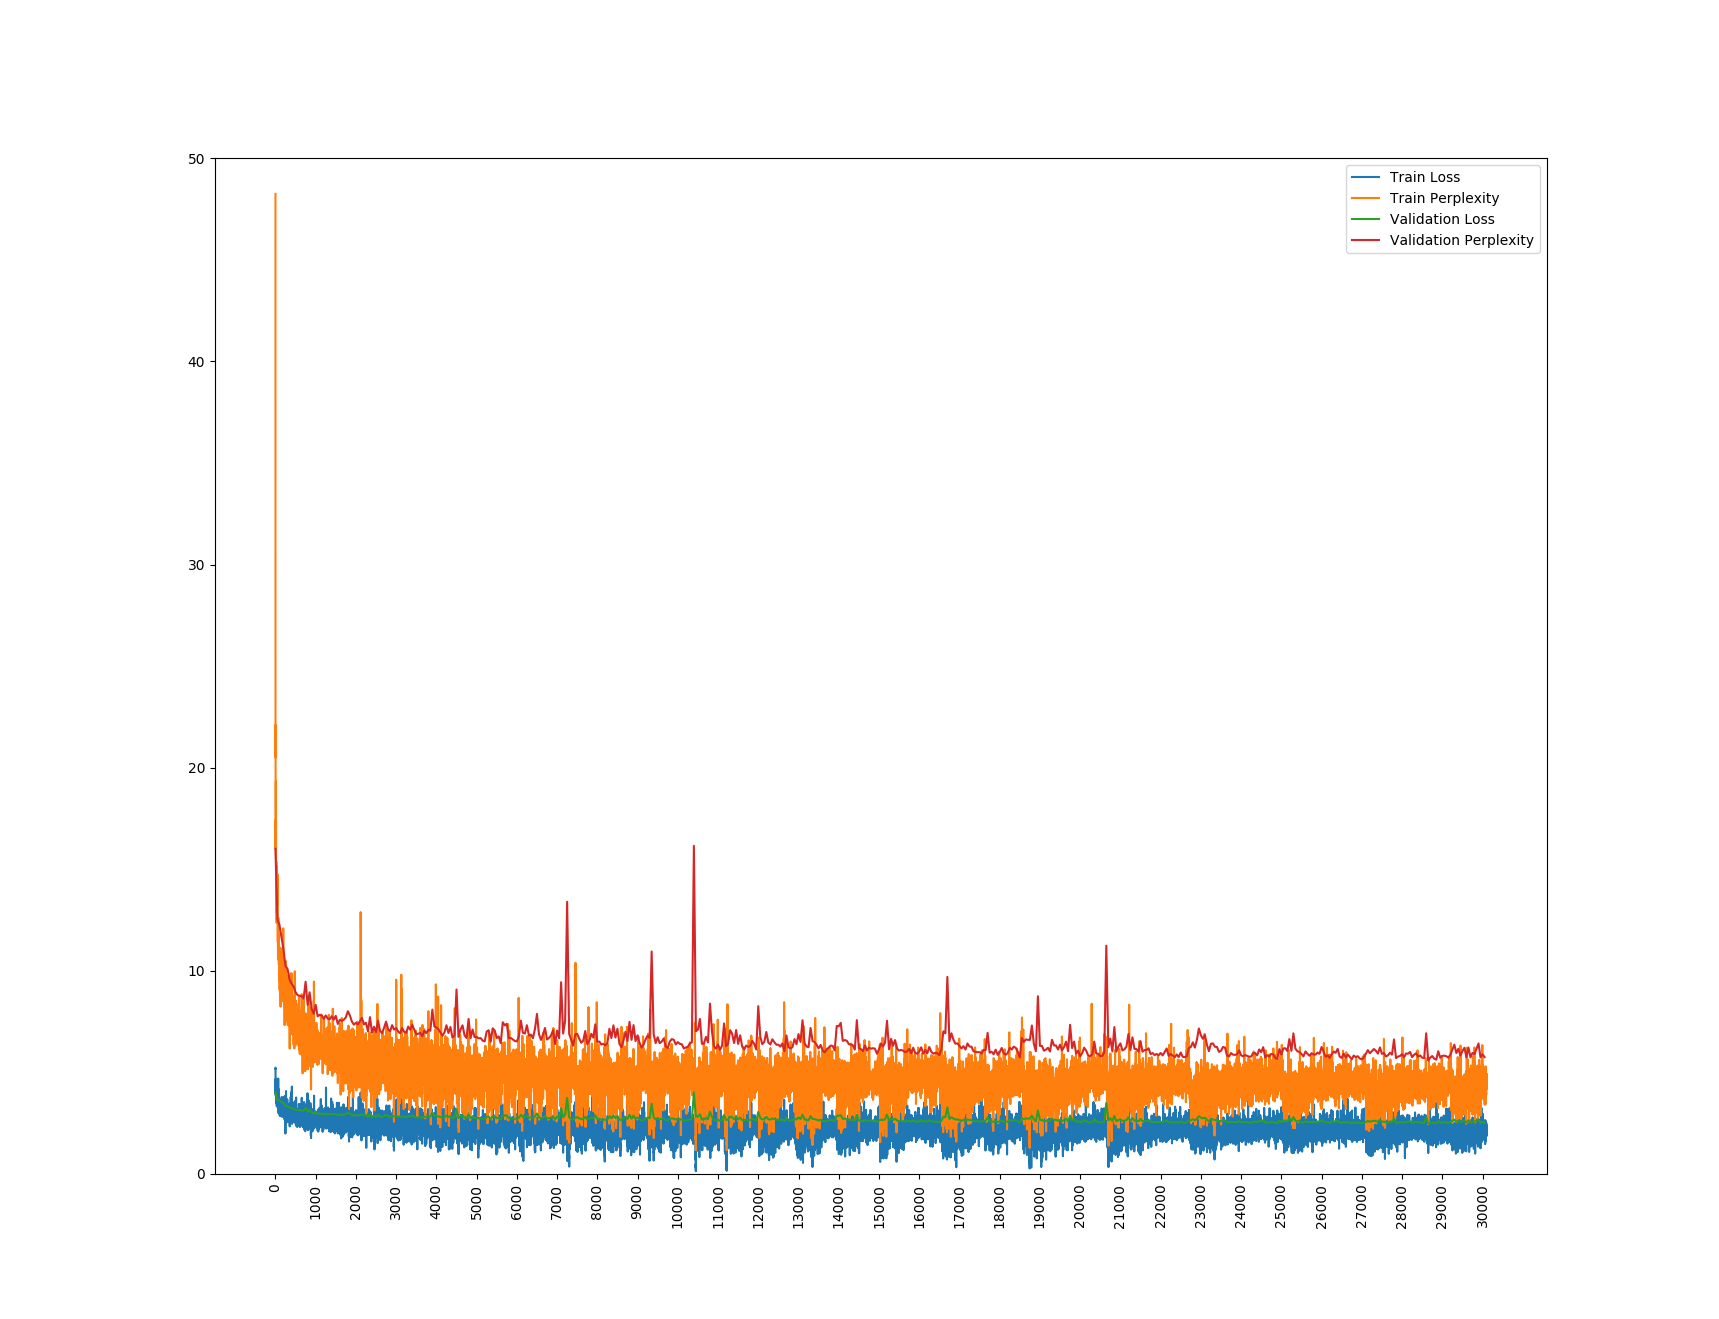
\includegraphics[width=\linewidth]{img/plots/opensubtitles_not_reversed/train_metrics.png}
	\caption{Development of the loss and perplexity values on the training and validation datasets throughout the training of the OpenSubtitles model. One tick on the x-axis is equal to $100,000$ batches processed.}
	\label{results:learning_process:metrics:opensubtitles}
\end{figure}

\paragraph{Reddit} The learning process of the Reddit model looks appropriate, but it also has a peculiarity, namely the dips in the training loss and perplexity. These dips occur about every $300,000$ to $400,000$ batches. They are also present in the development of the validation loss and perplexity, but are not as apparent as in the metrics on the training dataset. We currently cannot explain this behavior. We assume that this peculiarities are caused by the structure of the training dataset.\todo{Maybe explain a little bit more?} However, the variance is much smaller than with the OpenSubtitles model, which strengthens our argument that well-structured datasets are indeed favorable when training such systems as helps to avoid confusion due to perplexing samples.

\begin{figure}[H]
	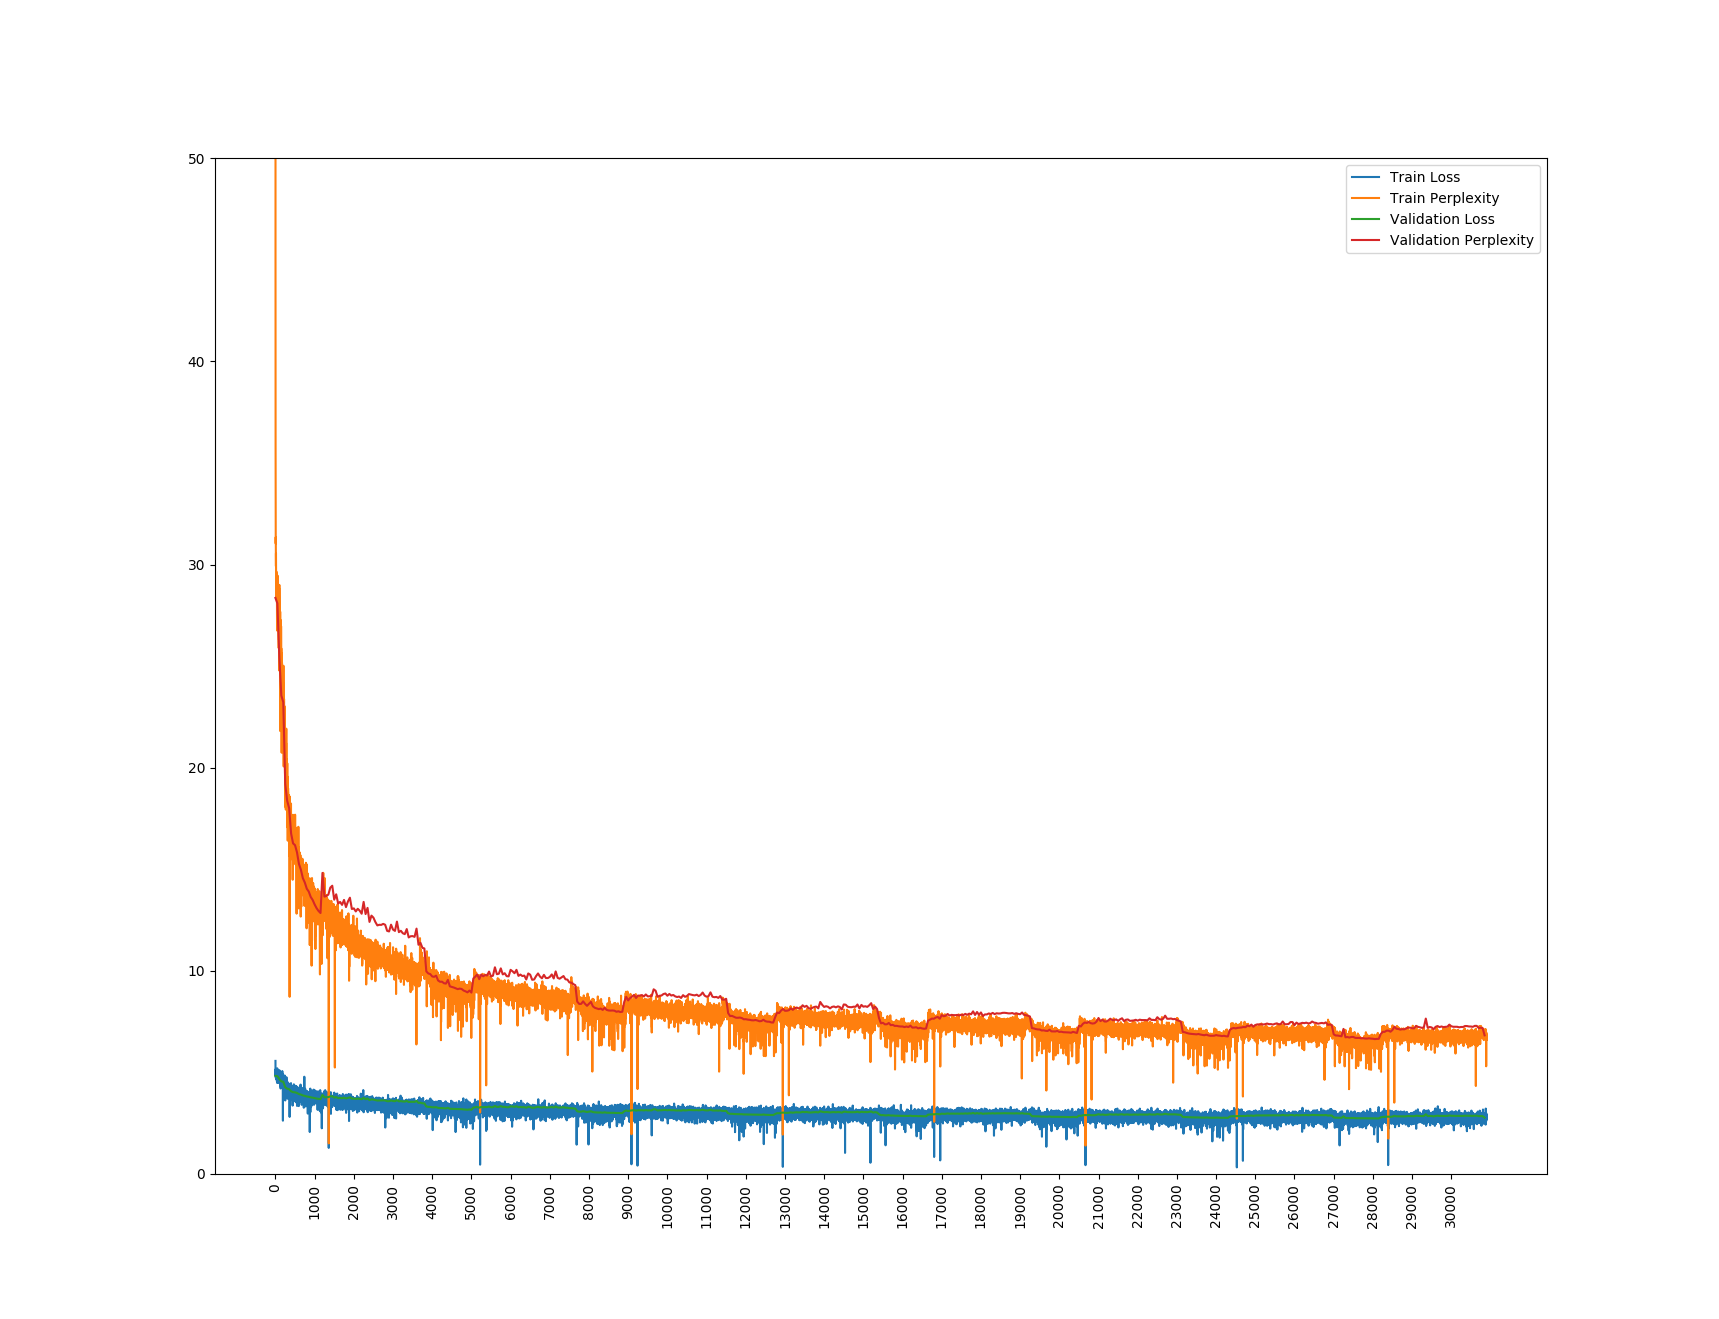
\includegraphics[width=\linewidth]{img/plots/reddit/train_metrics.png}
	\caption{Development of the loss and perplexity on the training and validation datasets throughout the training of the Reddit model. One tick on the x-axis is equal to $100,000$ batches processed.}
	\label{results:learning_process:metrics:reddit}
\end{figure} \todo{Wollen wir beobachtung mitteilne, dass wenn train perplex extrem sinkt, val perplex analog steigt?}

\paragraph{The Training Seems Successful} From the appearance of the plots, it looks like the training went fine for both models, as both of them exhibit decreasing loss and perplexity values. We see differences in how the models have evolved over the time span of the training, but we cannot derive any conclusion at the current time. After we have analyzed the training process, we are now focusing on the performance of the models on the test datasets.

\section{Performance on Test Datasets}
\label{results:performance_on_test_datasets}
After we have seen that the training process looks fine, we are going to assess the performance of these models on our test datasets. Here we use the same metrics as during the training, namely the cross-entropy loss and perplexity. We evaluate each model on the respective test dataset for each of the six snapshots we have created during training (see Chapter~\ref{methods:training}).

\paragraph{Surprising Results} The results on the test dataset are quite the opposite of the results of the training process, the performance for both of the models is
worsening over time. The results of the OpenSubtitles model (see Table~\ref{results:test_metrics:opensubtitles}) vary across the different snapshots, with the best result having a perplexity of $71.07$ and a loss of $6.15$ and derived from the evaluation of the first snapshot. Also, the best result of the Reddit model (see Table~\ref{results:test_metrics:reddit}) is achieved on the first snapshot with a perplexity of $169.14$, with all other snapshots having a worse perplexity.
\\
\begin{table}[H]
	\centering
	\begin{adjustbox}{max width=\textwidth}
		\begin{tabular}{l|cc}
			\toprule
			Snapshot & Test Loss & Test Perplexity\\
			\midrule
			0.5M & $6.1513$ & $71.0779$\\
			1.0M & $6.5314$ & $92.5000$\\
			1.5M & $7.3942$ & $168.2207$\\
			2.0M & $6.2134$ & $74.2035$\\
			2.5M & $6.3627$ & $82.2949$\\
			3.0M & $6.4647$ & $88.3205$\\
			\bottomrule
		\end{tabular}
	\end{adjustbox}
	\caption{Loss and perplexity values for each snapshot of the OpenSubtitles model when evaluating it with the test dataset.}
	\label{results:test_metrics:opensubtitles}
\end{table}

\begin{table}[H]
	\centering
	\begin{adjustbox}{max width=\textwidth}
		\begin{tabular}{l|cc}
			\toprule
			Snapshot & Test Loss & Test Perplexity\\
			\midrule
			0.5M & $7.4021$ & $169.1432$\\
			1.0M & $7.5477$ & $187.1090$\\
			1.5M & $7.5794$ & $191.2557$\\
			2.0M & $7.6288$ & $197.9190$\\
			2.5M & $7.6661$ & $203.1056$\\
			3.0M & $7.7885$ & $221.0843$\\
			\bottomrule
		\end{tabular}
	\end{adjustbox}
	\caption{Loss and perplexity values for each snapshot of the Reddit model when evaluating it with the test dataset.}
	\label{results:test_metrics:reddit}
\end{table}

This result contradicts with our expectation. Instead increasing loss values, we would have expected it to decrease in the same way as it did on the training and validation datasets. We assume, that this is related to the cross-entropy loss and hence the perplexity being not the best fit metrics to evaluate such models, especially in a conversational context where the variety of correct answers can be extensive. We have no explanation, why the values on the validation dataset are getting better over time. For this reason, we propose a third performance metric, namely the usage of Sent2Vec~\cite{Pgj:2017} embeddings, to measure the similarity between the expected and generated responses. Before we perform this analysis, we want to take a look at different samples from both models to show that they indeed improved over time, even though the results of the test metrics tell a different story.

\paragraph{Is Progress Achieved?} As the results of evaluating the models on the test dataset has shown, it seems that the models achieve a meaningful progress during the training. However, in the performance test, it appears like the models have become poorer over the course of the training. For this reason, we decided that we would like to evaluate the model manually and find out if the generated responses improve when using the six snapshots of the models. We have chosen four different input utterances, two for each model, and generated responses for each of the snapshots. The results can be seen in the Table~\ref{results:example_output:opensubtitles} for the OpenSubtitles model and Table~\ref{results:example_output:reddit} for the Reddit model.

\begin{table}[H]
	\centering
	\begin{adjustbox}{max width=\textwidth}
		\begin{tabularx}{\textwidth}{lX}
			\toprule
			Input: 	& \texttt{Do you like Joffrey from game of thrones?}\\
			\midrule
			0.5M: 	& \texttt{i m not sure if you re a fan of the movie ,}\\
			& \texttt{but i m not sure if you re a fan of the movie .}\\
			1.0M: 	& \texttt{i m not a fan of the game , but i m not sure if it s a game or not .}\\
			1.5M:	& \texttt{i do nt know what i m talking about .}\\
			2.0M:	& \texttt{i do nt }\\
			2.5M:	& \texttt{i do nt know what i m talking about .}\\
			3.0M:	& \texttt{i do nt know , i just do nt like him .}\\
			\midrule
			Input: 	& \texttt{Which movie can you recommend me?}\\
			\midrule
			0.5M: 	& \texttt{the}\\
			1.0M: 	& \texttt{the movie .}\\
			1.5M:	& \texttt{the one with the}\\
			2.0M:	& \texttt{the dark knight rises}\\
			2.5M:	& \texttt{the prestige}\\
			3.0M:	& \texttt{the movie}\\
			\bottomrule
		\end{tabularx}
	\end{adjustbox}
	\caption{Two exemplary dialogs with the Reddit model, one response per snapshot.}
	\label{results:example_output:reddit}
\end{table}

\begin{table}[H]
	\centering
	\begin{adjustbox}{max width=\textwidth}
		\begin{tabularx}{\textwidth}{lX}
			\toprule
			Input: 	& \texttt{Are you a man or a woman?}\\
			\midrule
			0.5M: 	& \texttt{no , no , no}\\
			1.0M: 	& \texttt{no}\\
			1.5M:	& \texttt{i m not a man}\\
			2.0M:	& \texttt{i m not a woman}\\
			2.5M:	& \texttt{i m a man}\\
			3.0M:	& \texttt{i m not a woman}\\
			\midrule
			Input: 	& \texttt{Why should it not be a good idea to improve you?}\\
			\midrule
			0.5M: 	& \texttt{no}\\
			1.0M: 	& \texttt{i don t know}\\
			1.5M:	& \texttt{because i love you}\\
			2.0M:	& \texttt{because i m a good man}\\
			2.5M:	& \texttt{i m just trying to make a good decision}\\
			3.0M:	& \texttt{i m not a good idea}\\
			\bottomrule
		\end{tabularx}
	\end{adjustbox}
	\caption{Two exemplary dialogs with the OpenSubtitles model, one response per snapshot.}
	\label{results:example_output:opensubtitles}
\end{table}

As seen in the examples above, there has indeed been an improvement in the answers from 0.5M and 1.0M to the better trained models, what stands in contradiction to the development of the performance of the models on the test datasets. We suspect from this result, again, that the cross-entropy loss and perplexity are not fit to assess if the responses are meaningful. As we have already described in Chapter~\ref{fundamentals:sent2vec_test}, we were aware of this potential issue; that is why we decided to use an additional metric, namely Sent2Vec embeddings, which we are going to use in the next Section.

\paragraph{Sent2Vec Analysis} As described in Chapter~\ref{fundamentals:sent2vec_test}, we leverage Sent2Vec embeddings for measuring the semantic similarity between the generated and expected responses on the test datasets. For this purpose, we have used the pretrained embeddings available on the GitHub page of the project\footnote{https://github.com/epfml/sent2vec}. We decided, that we use both the \emph{Twitter} and \emph{Wikipedia} embeddings for the assessment. The results can be seen in the Figures~\ref{results:sent2vec:opensubtitles:results} and~\ref{results:sent2vec:reddit:results}. It is obvious that both the Reddit and OpenSubtitles models perform better on the pretrained \emph{Wikipedia} embeddings in comparison to the pretrained \emph{Twitter} embeddings. This is probably related to the ``compressed'' language used when writing tweets (e.g. ``w/o'' instead of ``without''). In conclusion, the results of this analysis are dependent on the Sent2Vec embeddings, as expected. However, both results are poor, with the results from the Reddit model being about twice as good as results from the OpenSubtitles model (see Tables~\ref{results:sent2vec:opensubtitles:results_table} and~\ref{results:sent2vec:reddit:results_table}). The OpenSubtitles model starts with an average similarity of $0.167$ for the first snapshot and rises up to $0.204$ for the last snapshot. The Reddit model starts with an average value of $0.336$ for the first snapshot and increases to $0.359$ for the last snapshot. This means that the responses of the Reddit model match the expected responses much better from a semantic perspective as the responses of the OpenSubtitles model do. Our assumption is that this is, at least partially, related to the difference between written and spoken language found both in our datasets. It might be harder to learn from spoken language in our dataset as the conversations are extracted from movies, which leads to several subtle sources of information like pronunciation and body language being lost. Also, we are missing information about turn-taking, which makes the OpenSubtitles dataset more noisy. In summary, the results of both models are unsatisfactory, as the maximum achievable similarity is $1.0$.

\begin{figure}[H]
	\minipage{0.5\textwidth}
	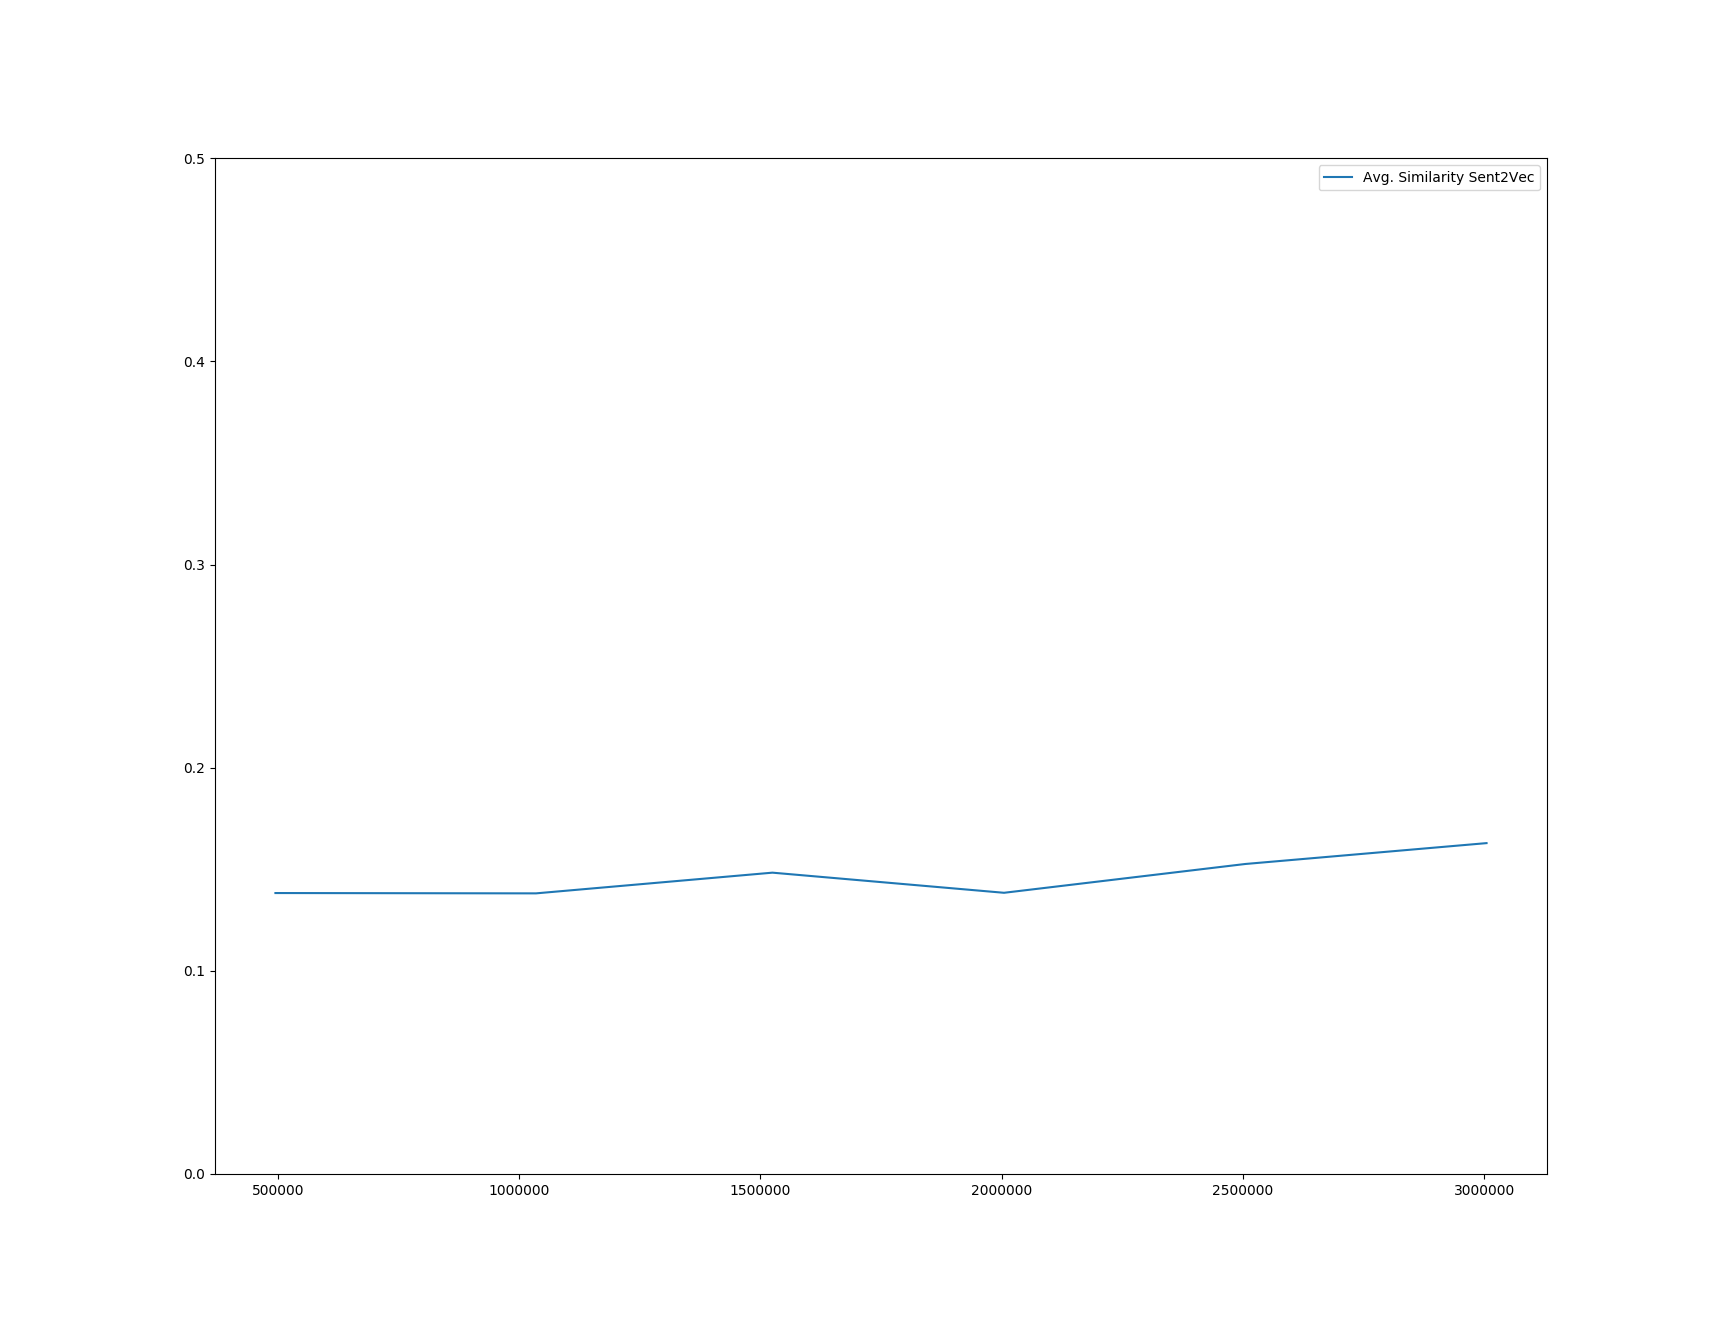
\includegraphics[width=\linewidth]{img/plots/opensubtitles_not_reversed/s2v_wiki_cosine_similarity.png}
	\centering
	\small
	\text{\emph{Wikipedia}}
	\endminipage\hfill
	\minipage{0.5\textwidth}
	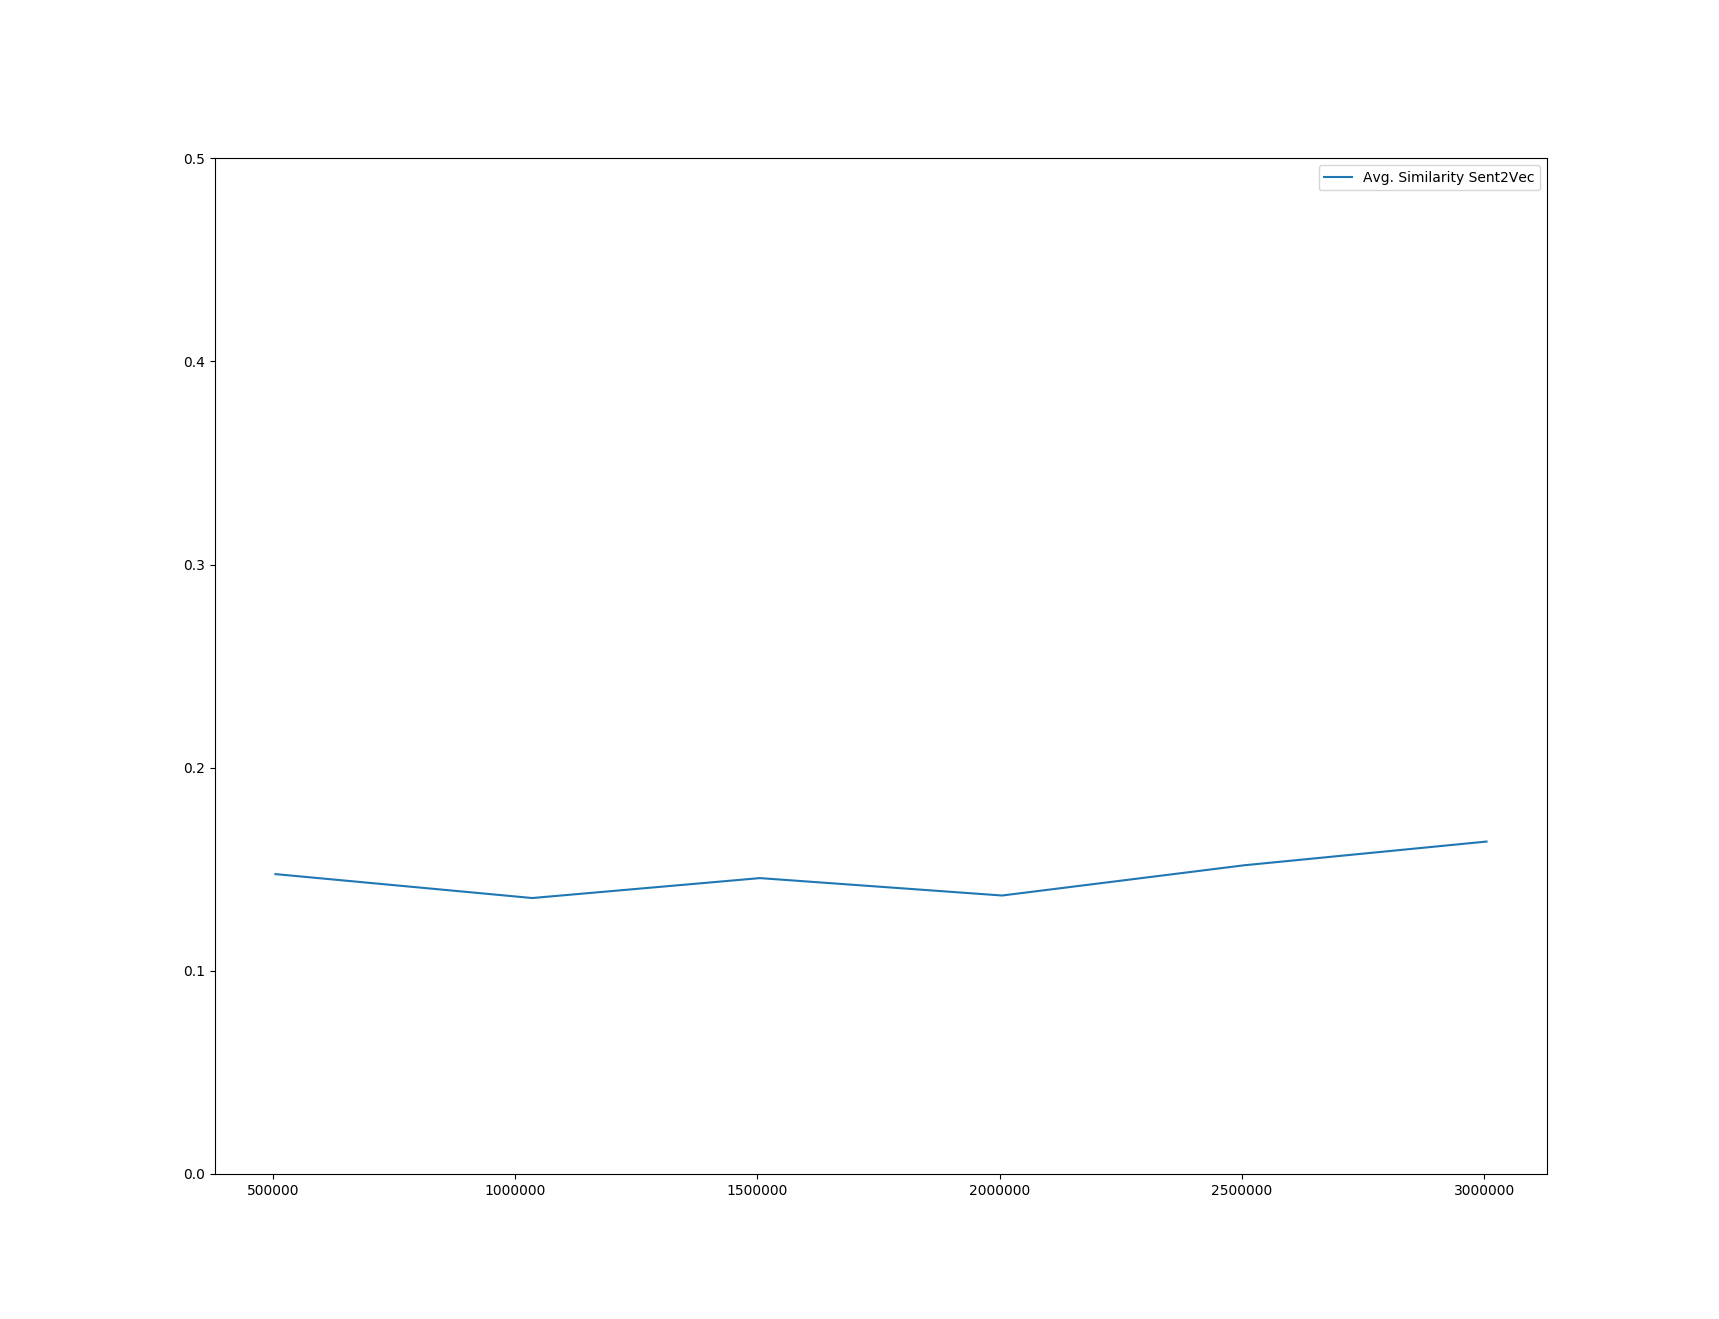
\includegraphics[width=\linewidth]{img/plots/opensubtitles_not_reversed/s2v_twitter_cosine_similarity.png}
	\centering
	\small
	\text{\emph{Twitter}}
	\endminipage\hfill
	\caption{Results of the evaluation with Sent2Vec on the outputs of the OpenSubtitles model when using the test dataset. The ticks on the x-axis show the different snapshots and the y-axis the average semantic similarity for each snapshot.}
	\label{results:sent2vec:opensubtitles:results}
\end{figure}

\begin{table}[H]
	\centering
	\begin{adjustbox}{max width=\textwidth}
		\begin{tabular}{lcc}
			\toprule
			Snapshot & Avg. Similarity (\emph{Wikipedia}) & Avg. Similarity (\emph{Twitter})\\
			\midrule
			0.5M & $0.16749$ & $0.13827$\\
			1.0M & $0.19111$ & $0.13811$\\
			1.5M & $0.19418$ & $0.14831$\\
			2.0M & $0.19176$ & $0.13840$\\
			2.5M & $0.20118$ & $0.15258$\\
			3.0M & $0.20452$ & $0.16285$\\
			\bottomrule
		\end{tabular}
	\end{adjustbox}
	\caption{The average similarities when using the Sent2Vec metric on the expected and generated responses from the OpenSubtitles model per snapshot.}
	\label{results:sent2vec:opensubtitles:results_table}
\end{table}

\begin{figure}[H]
	\minipage{0.5\textwidth}
	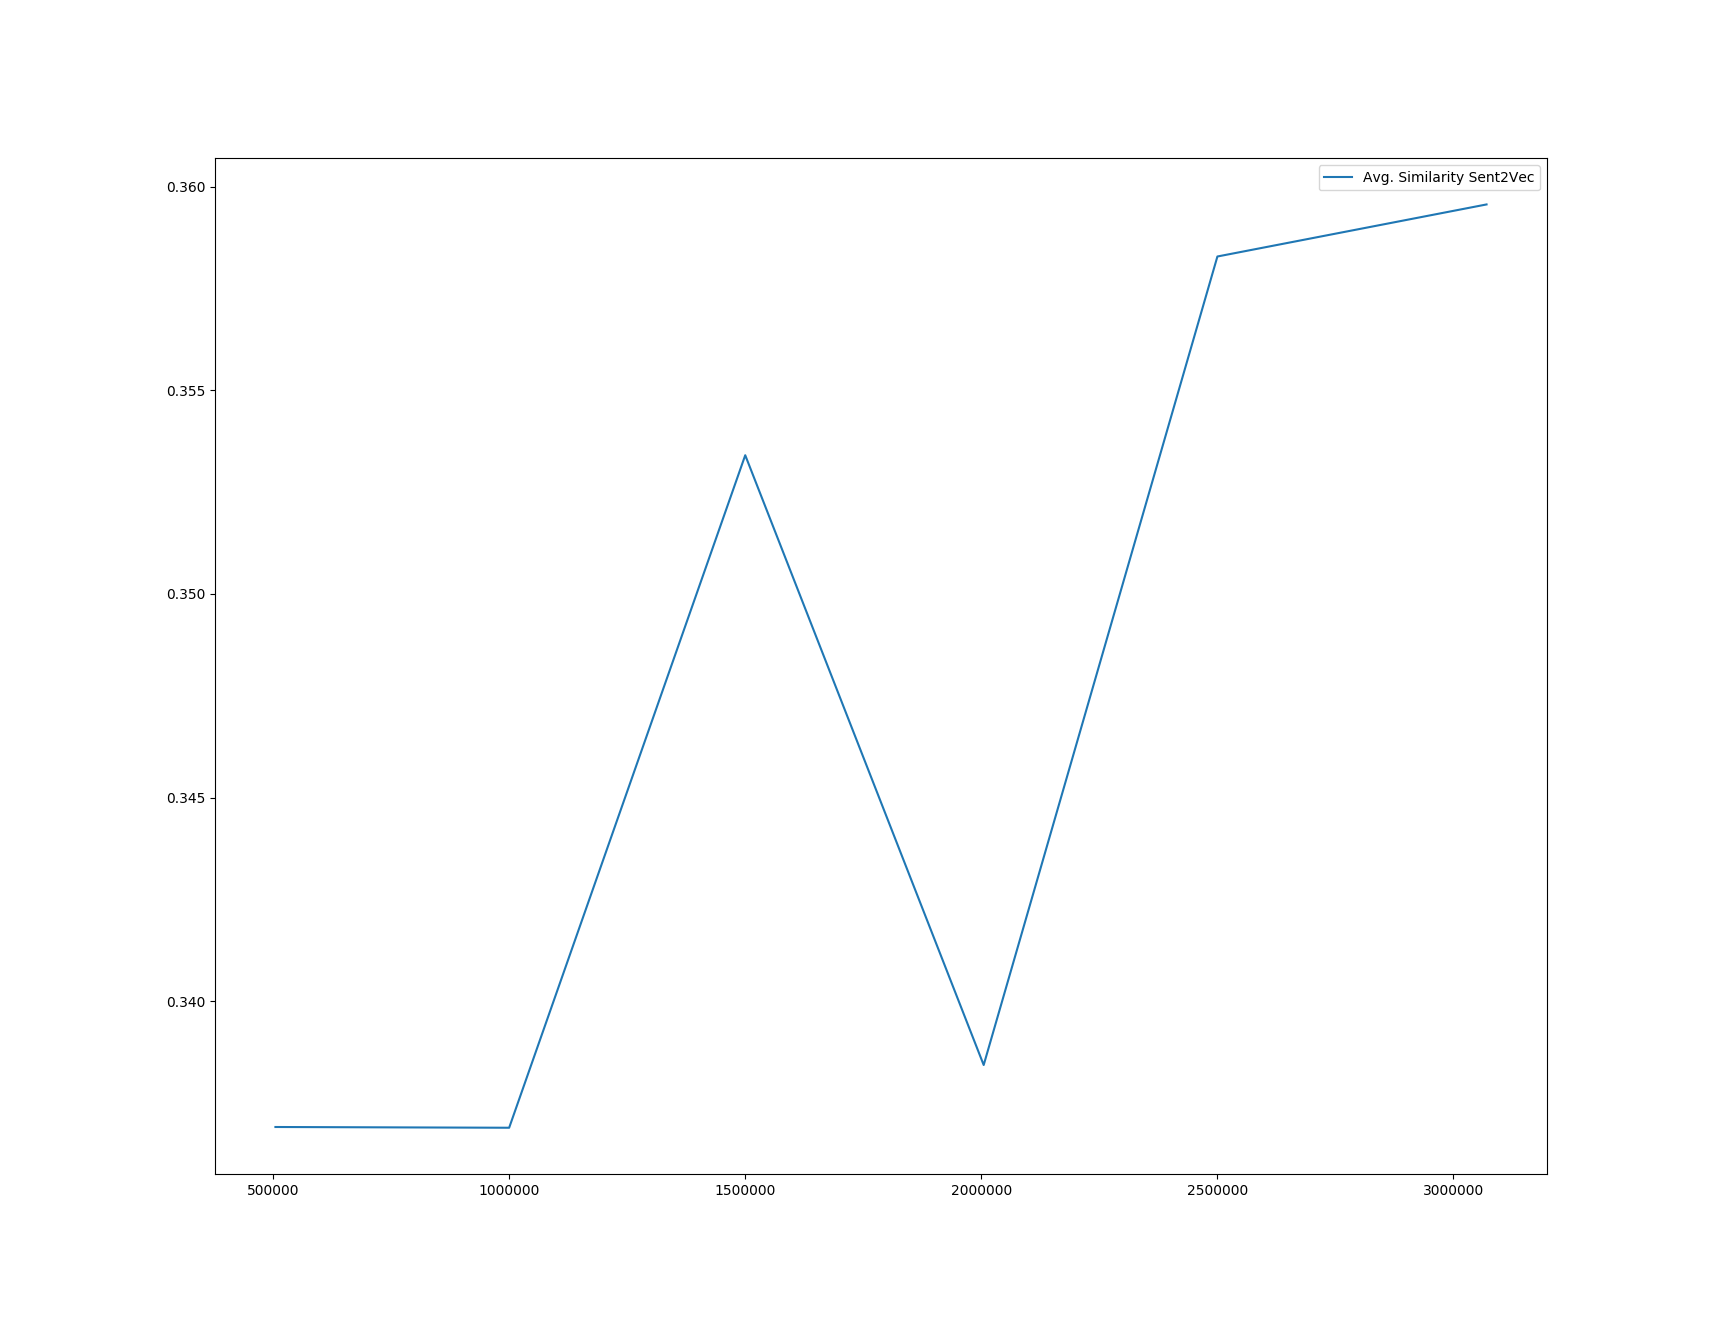
\includegraphics[width=\linewidth]{img/plots/reddit/s2v_wiki_cosine_similarity.png}
	\centering
	\small
	\text{\emph{Wikipedia}}
	\endminipage\hfill
	\minipage{0.5\textwidth}
	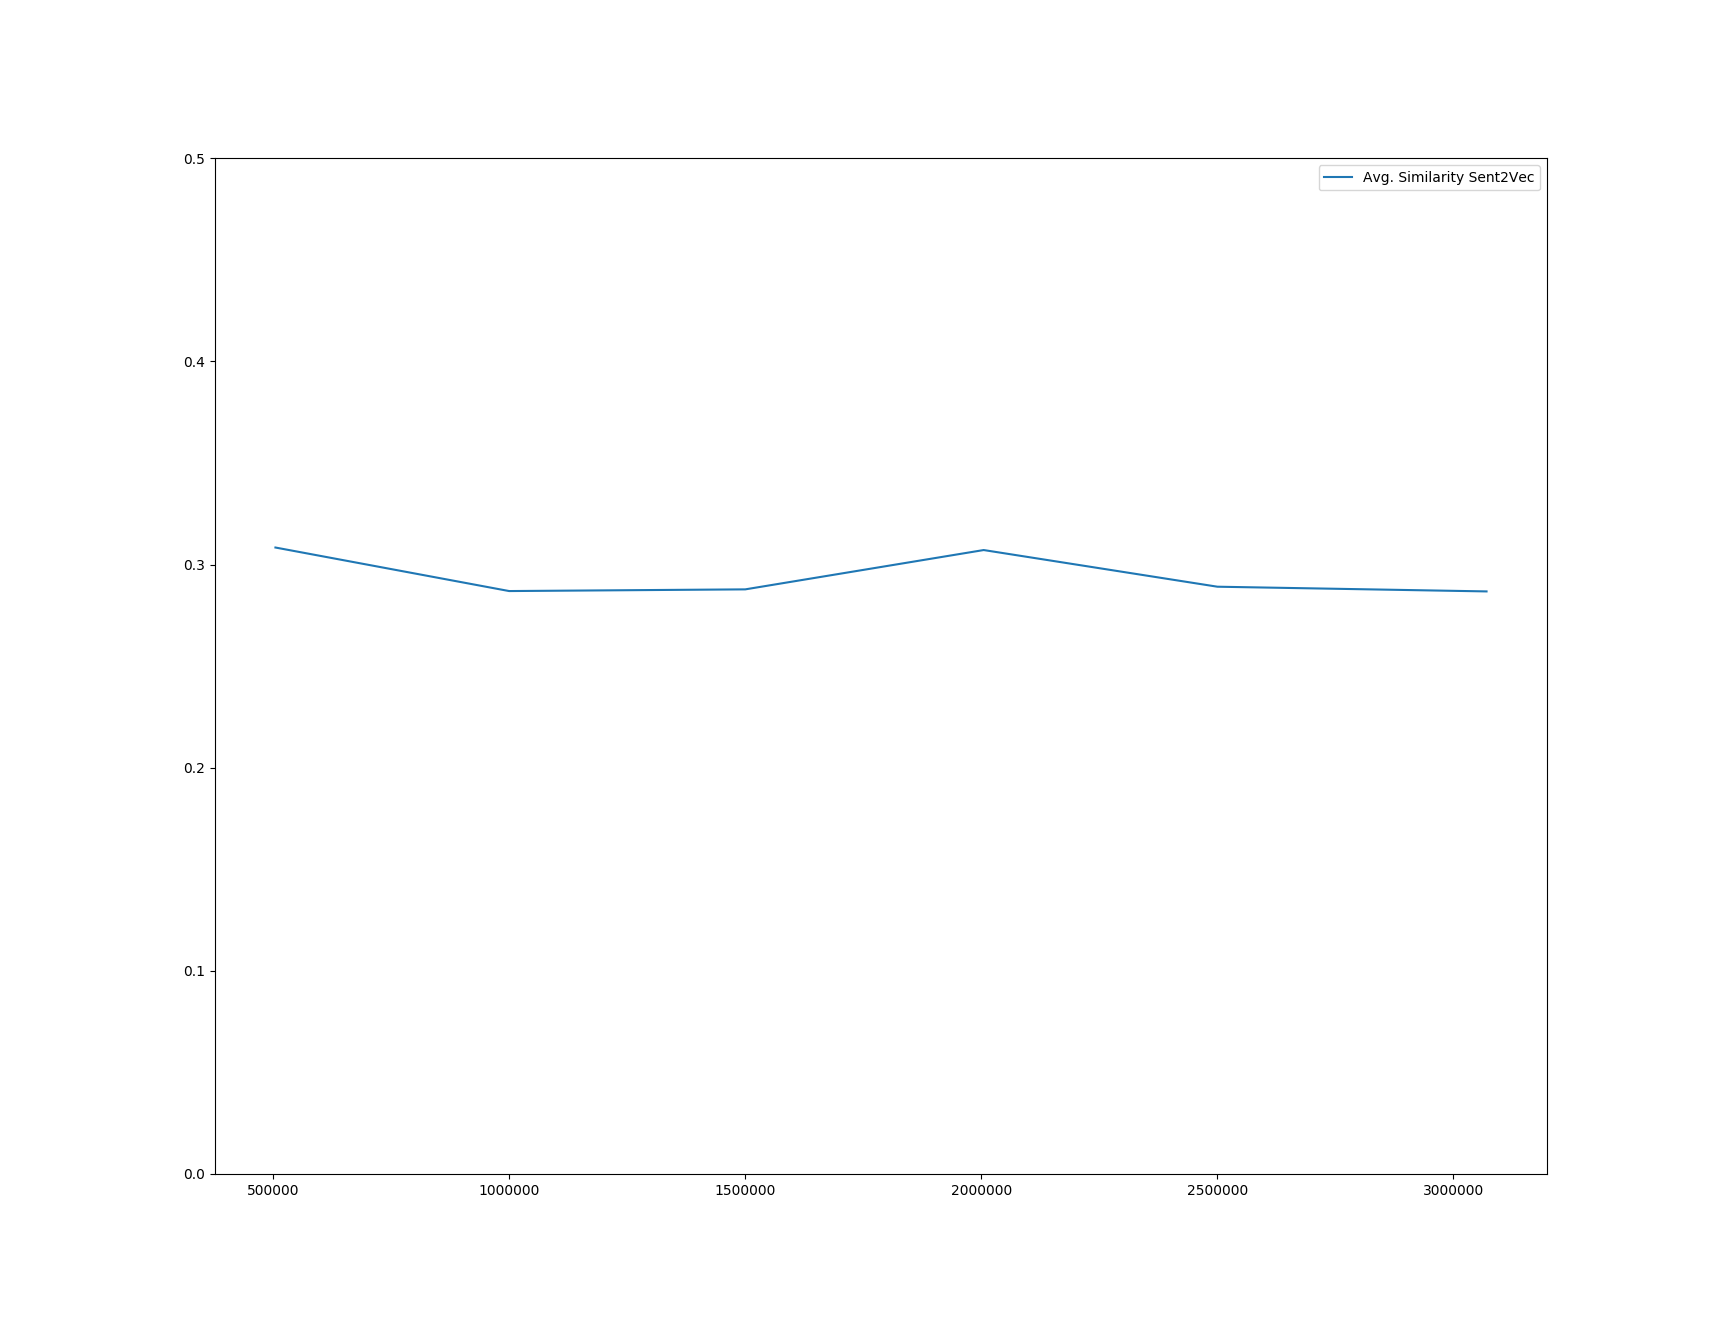
\includegraphics[width=\linewidth]{img/plots/reddit/s2v_twitter_cosine_similarity.png}
	\centering
	\small
	\text{\emph{Twitter}}
	\endminipage\hfill
	\caption{Results of the evaluation with Sent2Vec on the outputs of the Reddit model when using the test dataset. The ticks on the x-axis show the different snapshots and the y-axis the average semantic similarity for each snapshot.}
	\label{results:sent2vec:reddit:results}
\end{figure}
\begin{table}[H]
	\centering
	\begin{adjustbox}{max width=\textwidth}
		\begin{tabular}{lcc}
			\toprule
			Snapshot & Avg. Similarity (\emph{Wikipedia}) & Avg. Similarity (\emph{Twitter})\\
			\midrule
			0.5M & $0.33691$ & $0.30837$\\
			1.0M & $0.33689$ & $0.28694$\\
			1.5M & $0.35340$ & $0.28777$\\
			2.0M & $0.33843$ & $0.30713$\\
			2.5M & $0.35828$ & $0.28908$\\
			3.0M & $0.35956$ & $0.28676$\\
			\bottomrule
		\end{tabular}
	\end{adjustbox}
	\caption{The average similarities when using the Sent2Vec metric on the expected and generated responses from the Reddit model per snapshot.}
	\label{results:sent2vec:reddit:results_table}
\end{table}

\paragraph{Generic Response Are a Problem} A potential reason for the poor results when using the Sent2Vec metric could be based on our observation that both models often generate generic responses (e.g. ``i don t know'', ``i m not sure what you re saying''). Our first idea to analyze this is to see what kind of sentences the models produce with the inputs of the test datasets. We did an analysis on the generated responses and quickly noticed that there are a few sentences, which are often predicted by the models (see Tables~\ref{results:test_performance:opensubtitles_sample_outputs} and~\ref{results:test_performance:reddit_sample_outputs}). As one can see in the column \emph{Percentage}, these generic responses take up a great share of all the generated responses. The top 10 responses from the OpenSubtitles model make up 45.77\% of all outputs, where the same for the Reddit only sums up to 33.02\% of all outputs.
\\
\begin{table}[H]
	\centering
	\begin{adjustbox}{max width=\textwidth}
		\begin{tabularx}{\textwidth}{lcc}
			\toprule
			Sentence & Occurrence Frequency & Percentage \\ \midrule
			\texttt{i m not gon na let you go} & 41853 & 16.74\%\\
			\texttt{i m not sure i can trust you} & 21263 & 8.51\%\\
			\texttt{i m not gon na say anything} & 9163 & 3.67\%\\
			\texttt{i m not gon na let that happen} & 7426 & 2.97\%\\
			\texttt{i m sorry} & 7235 & 2.89\\
			\texttt{you re not gon na believe this} & 7068 & 2.83\%\\
			\texttt{you re not gon na believe me} & 6878 & 2.75\%\\
			\texttt{i m not gon na hurt} you & 4829 & 1.93\%\\
			\texttt{i m not a fan} & 4468 & 1.79\%\\
			\texttt{i m not sure} & 4215 & 1.69\%\\
			\midrule
			Summed up & 114408 & 45.77\%\\
			\midrule
			\midrule
			Total Sentences Count & 249984 & 100.00\%\\
			\bottomrule
		\end{tabularx}
	\end{adjustbox}
	\caption{Top 10 most generated responses with respective occurrence frequencies when using the last OpenSubtitles snapshot and the test dataset.}
	\label{results:test_performance:opensubtitles_sample_outputs}
\end{table}

\begin{table}[H]
	\centering
	\begin{adjustbox}{max width=\textwidth}
		\begin{tabular}{lcc}
			\toprule
			Sentence & Occurrence Frequency & Percentage\\ \midrule
			\texttt{i m not sure if i m being sarcastic or not .} & 17486 & 7.00\%\\
			\texttt{i think it s a bit of a stretch .} & 13058 & 5.22\%\\
			\texttt{i m not sure if you re being sarcastic or not .} & 11647 & 4.66\%\\
			\texttt{i m not sure if i m a <unknown> or not .} & 8307 & 3.32\%\\
			\texttt{i m not sure if you re joking or not .} & 7932 & 3.17\%\\
			\texttt{i was thinking the same thing .} & 7579 & 3.03\%\\
			\texttt{<unknown>} & 6210 & 2.48\%\\
			\texttt{i m not sure if i m going to watch this or not .} & 4257 & 1.70\%\\
			\specialcell{\texttt{i m not sure if i m a fan of the show , but i m}\\\texttt{pretty sure that s a <unknown> .}} & 3232 & 1.29\%\\
			\texttt{i m not sure if i m going to watch it or not .} & 3079 & 1.23\%\\
			\midrule
			Summed up & 82797 & 33.02\%\\
			\midrule
			\midrule
			Total Amount Sentences & 249984 & 100.00\%\\
			\bottomrule
		\end{tabular}
	\end{adjustbox}
	\caption{Top 10 most generated sentences with respective occurrence frequencies when using the last Reddit snapshot and the test dataset. The meaning of the \textless unknown\textgreater \ token is described in \ref{data:word_coverage}.}
	\label{results:test_performance:reddit_sample_outputs}
\end{table}

\paragraph{Does Filtering of Generic Responses Help?} As seen in the Tables above, there are certain responses which are generated a lot of time and are pretty generic and meaningless in most contexts. Because of that, we think it would be a good idea to evaluate the models under the Sent2Vec metric one more time, but this time with the top $n$ most generated responses filtered out. We do this expecting that the generic sentences are the cause of the small average similarities. The results of the analysis with the top $n$ most generated responses filtered out is shown in Table~\ref{results:sent2vec:opensubtitles:top_n_results_table} and~\ref{results:sent2vec:reddit:top_n_results_table}. For this analysis, we only use the \emph{Wikipedia} embeddings as it has shown a better performance for both of our models before.
\\
\begin{table}[H]
	\centering
	\begin{adjustbox}{max width=\textwidth}
		\begin{tabular}{lccc}
			\toprule
			Snapshot & $n = 1$ & $n = 5$ & $n = 10$\\
			\midrule
			0.5M & $0.16679$ & $0.16804$ & $0.16854$\\
			1.0M & $0.19329$ & $0.19394$ & $0.19575$\\
			1.5M & $0.19491$ & $0.19519$ & $0.19539$\\
			2.0M & $0.19215$ & $0.19192$ & $0.19284$\\
			2.5M & $0.20102$ & $0.20127$ & $0.20182$\\
			3.0M & $0.20431$ & $0.20547$ & $0.20568$\\
			\bottomrule
		\end{tabular}
	\end{adjustbox}
	\caption{The average similarities when applying the Sent2Vec metric on the expected and generated responses on the test dataset when filtering out the top $n$ most generated responses for the OpenSubtitles model.}
	\label{results:sent2vec:opensubtitles:top_n_results_table}
\end{table}

\begin{table}[H]
	\centering
	\begin{adjustbox}{max width=\textwidth}
		\begin{tabular}{lccc}
			\toprule
			Snapshot & $n = 1$ & $n = 5$ & $n = 10$\\
			\midrule
			0.5M & $0.33772$ & $0.34101$ & $0.34589$\\
			1.0M & $0.34225$ & $0.34238$ & $0.34295$\\
			1.5M & $0.35383$ & $0.35605$ & $0.35564$\\
			2.0M & $0.34008$ & $0.34009$ & $0.34198$\\
			2.5M & $0.35937$ & $0.36142$ & $0.36175$\\
			3.0M & $0.36043$ & $0.35950$ & $0.36313$\\
			\bottomrule
		\end{tabular}
	\end{adjustbox}
	\caption{The average similarities when applying the Sent2Vec metric on the expected and generated responses on the test dataset when filtering out the top $n$ most generated responses for the Reddit model.}
	\label{results:sent2vec:reddit:top_n_results_table}
\end{table}

As seen above, the filtering of the most used responses does not help significantly when it comes to the Sent2Vec evaluation. We currently cannot say if this problem is just apparent in our specific use-case or inherent to the metric itself. To come to a definitive conclusion, we would have to investigate further by using this metric for evaluating other models.

\paragraph{Mixed Feelings about Performance Metrics} As seen in this Chapter, the performance metrics we use to evaluate the models tell us an indifferent story about the resulting models. On one hand, we see that the training performed acceptable and the learning process ran as expected. However, as we subsequently test these trained models against the test datasets with the different metrics, it looks like the performance decreased over the duration of the training. Our subjective opinion could not confirm this after we were ``talking'' to both models for an extensive period of time. We think the biggest problem for the evaluation is the large portion of generic responses both models seem to generate. To identify the cause of this generic responses, we will now analyze the development of the language model while training, trying to establish a connection between the language model in the datasets and the ones produced by the models.

\section{Development of Language Model}
\label{results:development_language_model}
In this Chapter, we are investigating into the language models produced by the training and try to identify a reason for the generic responses.

\subsection{Uni- and Bi-Gram Distributions over Time}
Initially, we are comparing the uni- and bi-gram distributions of the training datasets with the distributions produced when evaluating the models with the test datasets. For this purpose, we have generated uni-gram and bi-gram statistics using \texttt{nltk} on the training datasets and outputs generated by the models.

\paragraph{OpenSubtitles} The OpenSubtitles has the most evenly spread distribution (see Figure~\ref{results:bigram:distributions:opensubtitles}) when using the first snapshot (i.e. 0.5M). We observe a pattern when we look at all distributions of the OpenSubtitles model. At the beginning, it starts with a rather evenly spread distribution of uni- and bi-grams. As the training proceeds, these distributions shift to a more right-leaned when looking at the distributions for the snapshot 1.0M. The distributions then return to be more evenly distributed again. This pattern repeats until the last snapshot, with one being evenly distributed whereas the next is then again more right-leaned.

We cannot provide a complete explanation for this behavior, but we assume that this is related to the rather noisy dataset we are using for the OpenSubtitles model. This probably leads to the model being confused, rejecting what it has already learned and trying to fit to the newly provided samples. Because of the fact that we cannot fully explain this behavior, we are going to analyze the development of the diversity of the uni-, bi-gram and sentences over the course of the training.

The behavior of the uni-gram distributions develops in a similar way, therefore we documented these visualizations in the Appendix~\ref{appendix:unigram_distributions}.

\begin{figure}[H]
	\minipage{0.5\textwidth}
	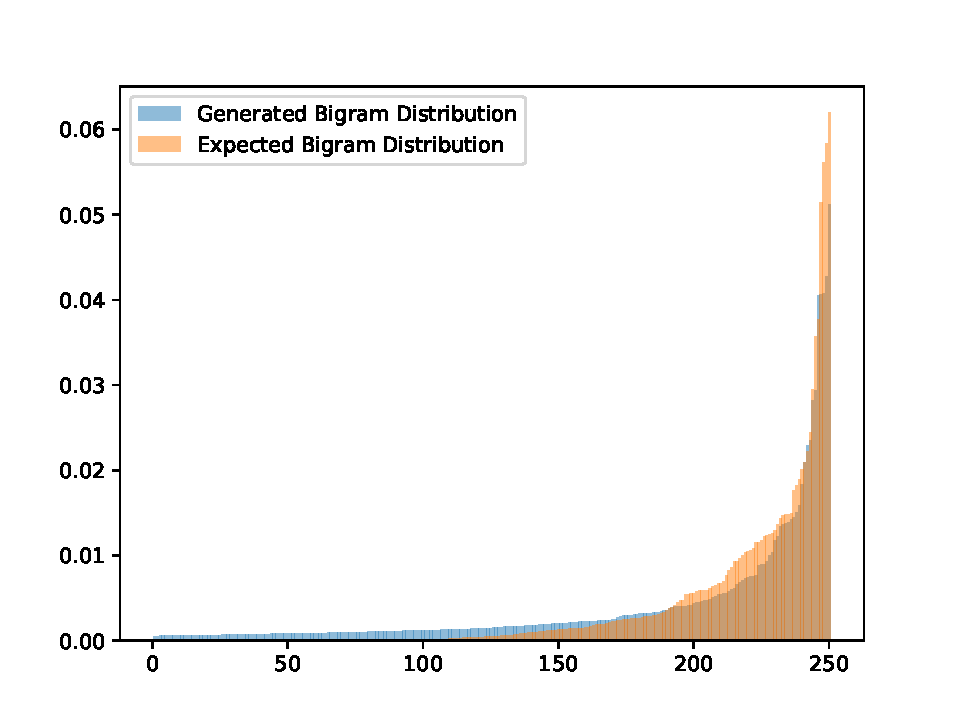
\includegraphics[width=\linewidth]{img/plots/opensubtitles_not_reversed/bigram_distribution_comparison_step_500000.pdf}
	\centering
	\small
	\text{Snapshot 0.5M}
	\endminipage\hfill
	\minipage{0.5\textwidth}
	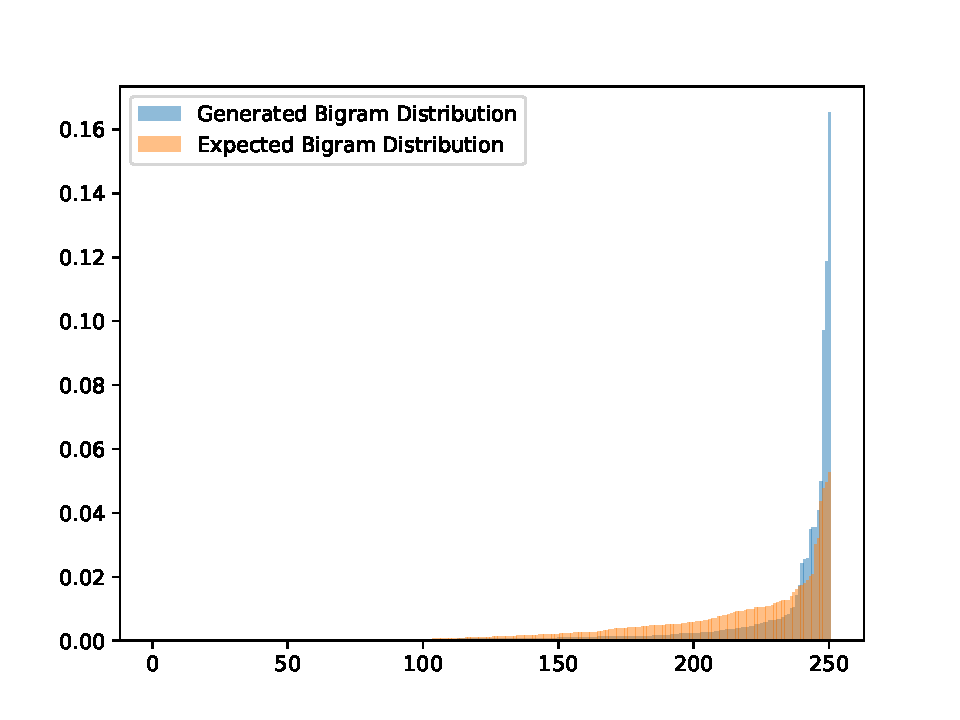
\includegraphics[width=\linewidth]{img/plots/opensubtitles_not_reversed/bigram_distribution_comparison_step_1000000.pdf}
	\centering
	\small
	\text{Snapshot 1.0M}
	\endminipage\hfill
	\minipage{0.5\textwidth}
	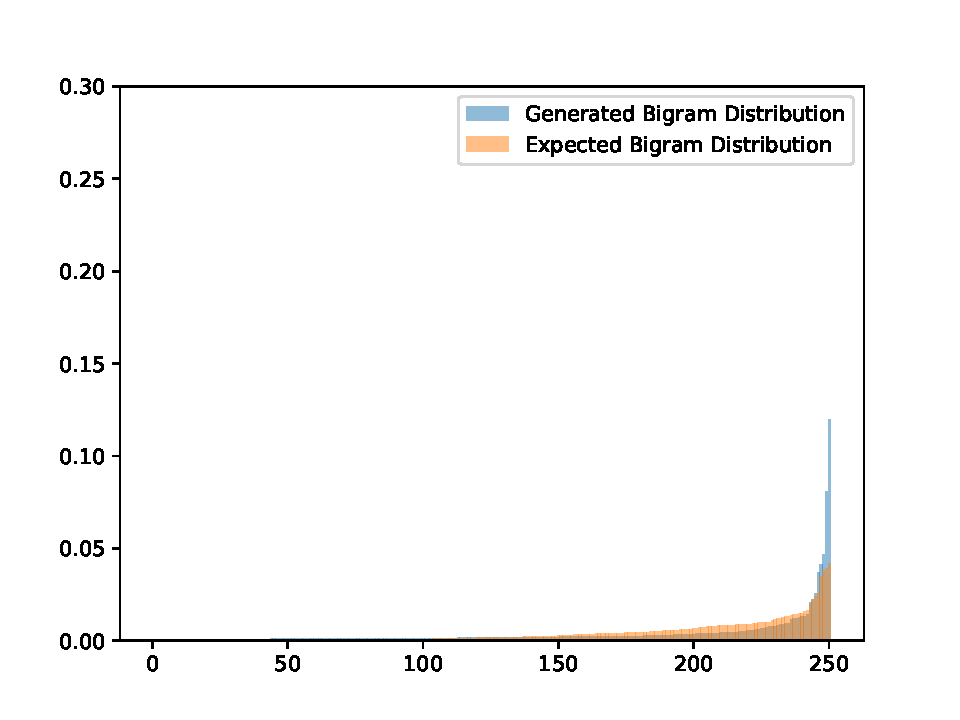
\includegraphics[width=\linewidth]{img/plots/opensubtitles_not_reversed/bigram_distribution_comparison_step_1500000.pdf}
	\centering
	\small
	\text{Snapshot 1.5M}
	\endminipage\hfill
	\minipage{0.5\textwidth}
	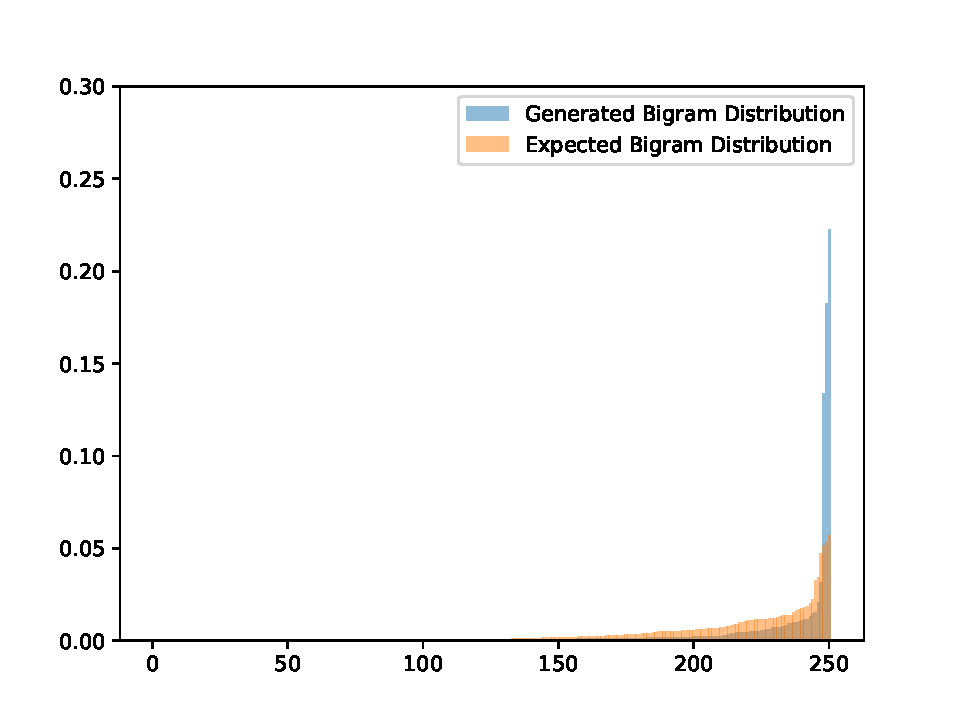
\includegraphics[width=\linewidth]{img/plots/opensubtitles_not_reversed/bigram_distribution_comparison_step_2000000.pdf}
	\centering
	\small
	\text{Snapshot 2.0M}
	\endminipage\hfill
	\minipage{0.5\textwidth}
	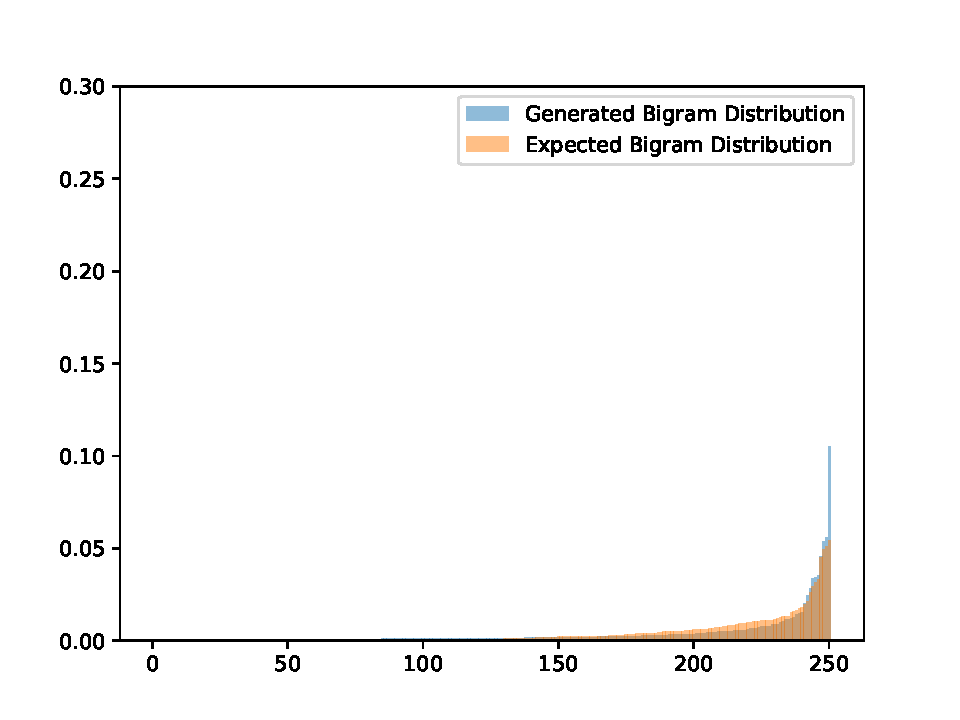
\includegraphics[width=\linewidth]{img/plots/opensubtitles_not_reversed/bigram_distribution_comparison_step_2500000.pdf}
	\centering
	\small
	\text{Snapshot 2.5M}
	\endminipage\hfill
	\minipage{0.5\textwidth}
	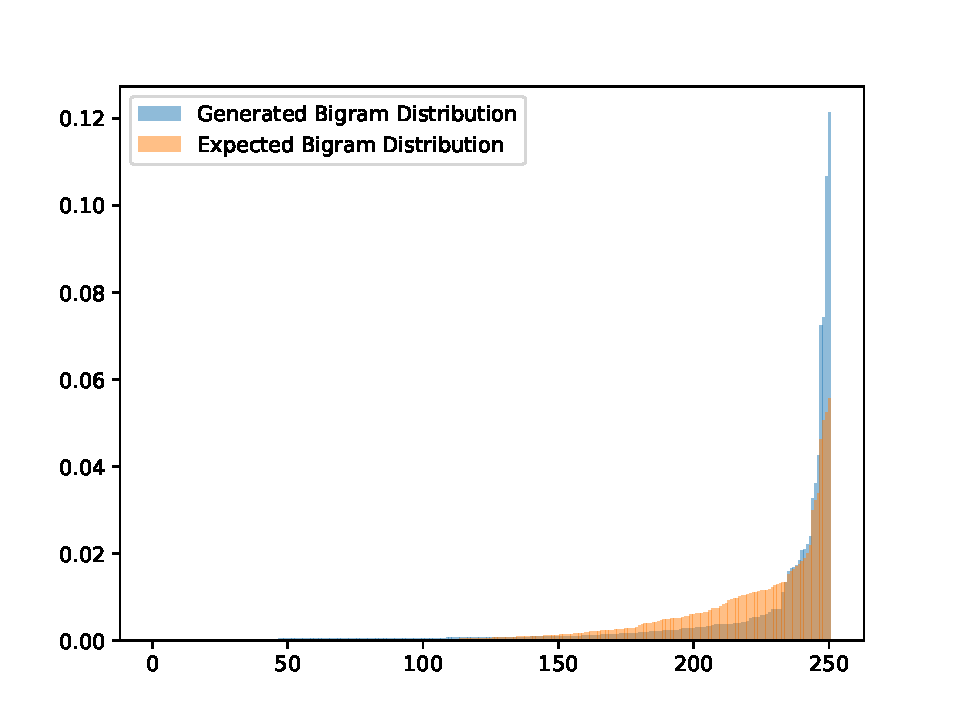
\includegraphics[width=\linewidth]{img/plots/opensubtitles_not_reversed/bigram_distribution_comparison_step_3000000.pdf}
	\centering
	\small
	\text{Snapshot 3.0M}
	\endminipage\hfill
	\caption{Comparison of the distributions of the top 250 most used bi-grams for the responses of the OpenSubtitles model (orange) when using the test dataset and the distribution within the training dataset (blue). The distributions are compared for each snapshot available.}
	\label{results:bigram:distributions:opensubtitles}
\end{figure}

\paragraph{Reddit} The distributions for the Reddit model reveal an interesting development (see Figure~\ref{results:bigram:distributions:reddit}). In the beginning, same as with the OpenSubtitles, the distributions are evenly spread. However, as the training continues, the distributions increasingly better fit the expected distributions, until the fit reaches the highest overlap when using the 1.5M and 2.0M snapshots. From this point onwards, the distributions start to drift apart again. This coincides in our opinion, that the Reddit model is at its performance peak when using the snapshot 2.0M. This is probably associated with the fact that we are doing more than two epochs over the full dataset. From the snapshot 2.0M on, the model itself starts to become worse, as the diversity and quality of the responses starts to decline. We are going to analyze this assumption below.

The behavior of the uni-gram distributions develops in a similar way, therefore we documented these visualizations in the Appendix~\ref{appendix:unigram_distributions}.

\begin{figure}[H]
	\minipage{0.5\textwidth}
	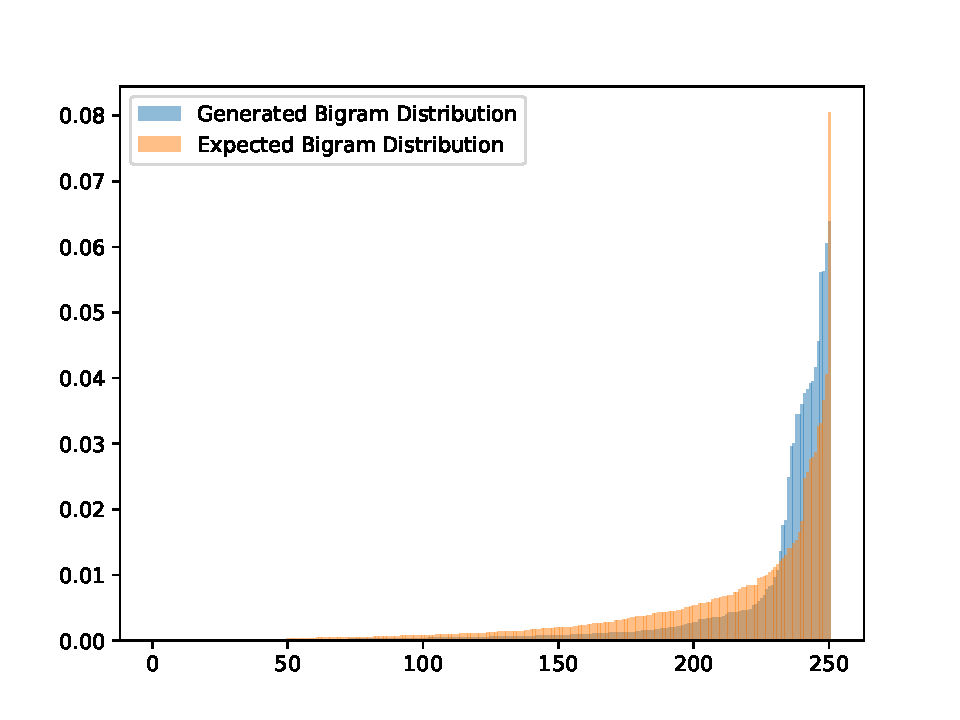
\includegraphics[width=\linewidth]{img/plots/reddit/bigram_distribution_comparison_step_500000.pdf}
	\centering
	\small
	\text{Snapshot 0.5M}
	\endminipage\hfill
	\minipage{0.5\textwidth}
	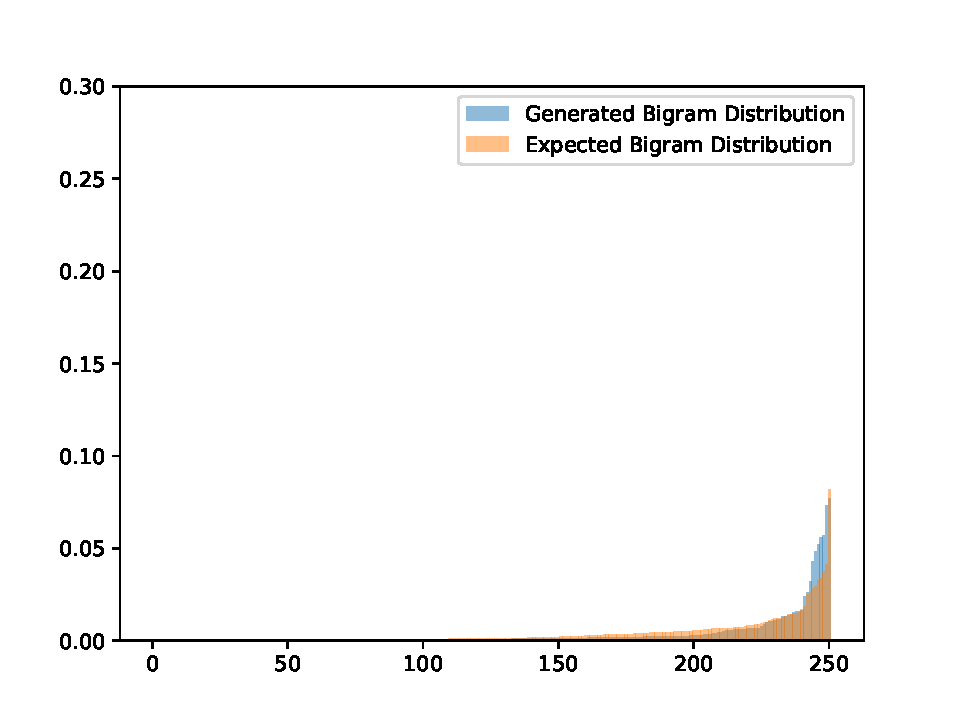
\includegraphics[width=\linewidth]{img/plots/reddit/bigram_distribution_comparison_step_1000000.pdf}
	\centering
	\small
	\text{Snapshot 1.0M}
	\endminipage\hfill
	\minipage{0.5\textwidth}
	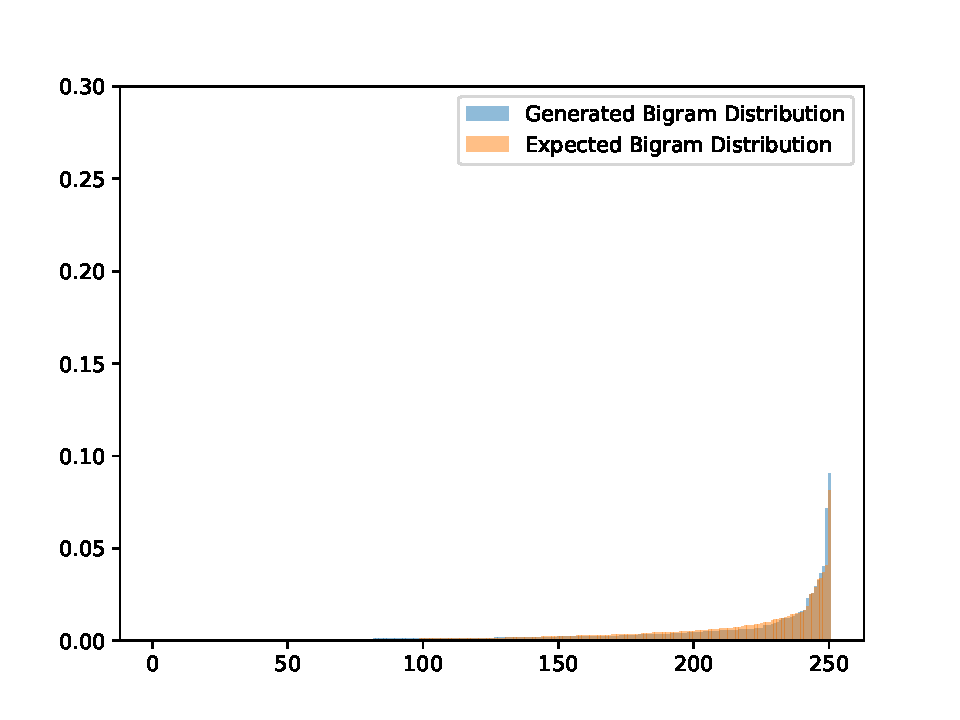
\includegraphics[width=\linewidth]{img/plots/reddit/bigram_distribution_comparison_step_1500000.pdf}
	\centering
	\small
	\text{Snapshot 1.5M}
	\endminipage\hfill
	\minipage{0.5\textwidth}
	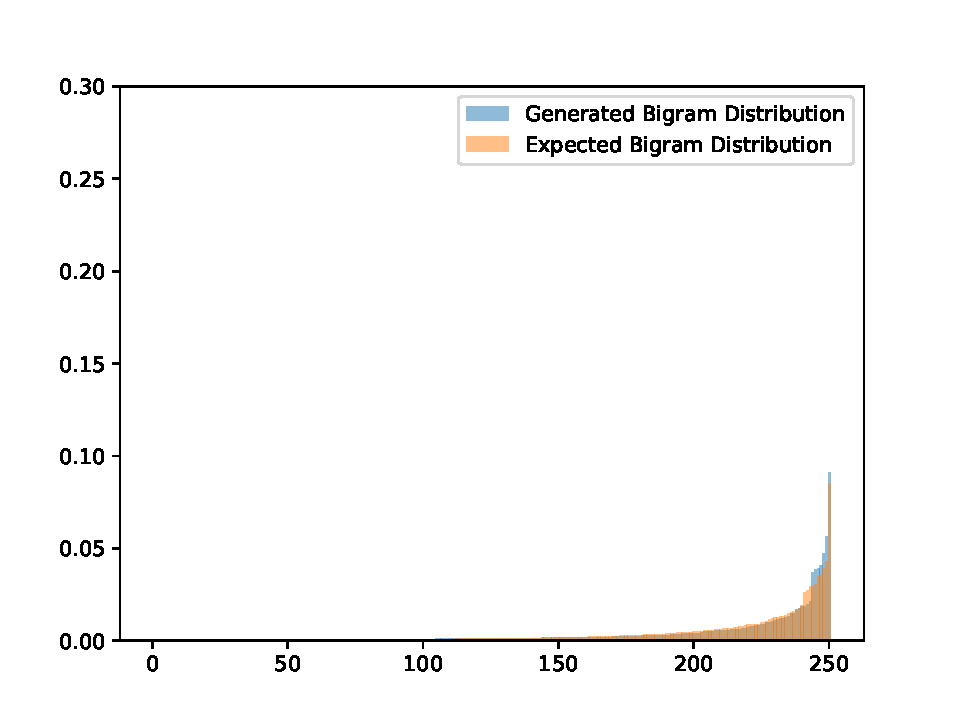
\includegraphics[width=\linewidth]{img/plots/reddit/bigram_distribution_comparison_step_2000000.pdf}
	\centering
	\small
	\text{Snapshot 2.0M}
	\endminipage\hfill
	\minipage{0.5\textwidth}
	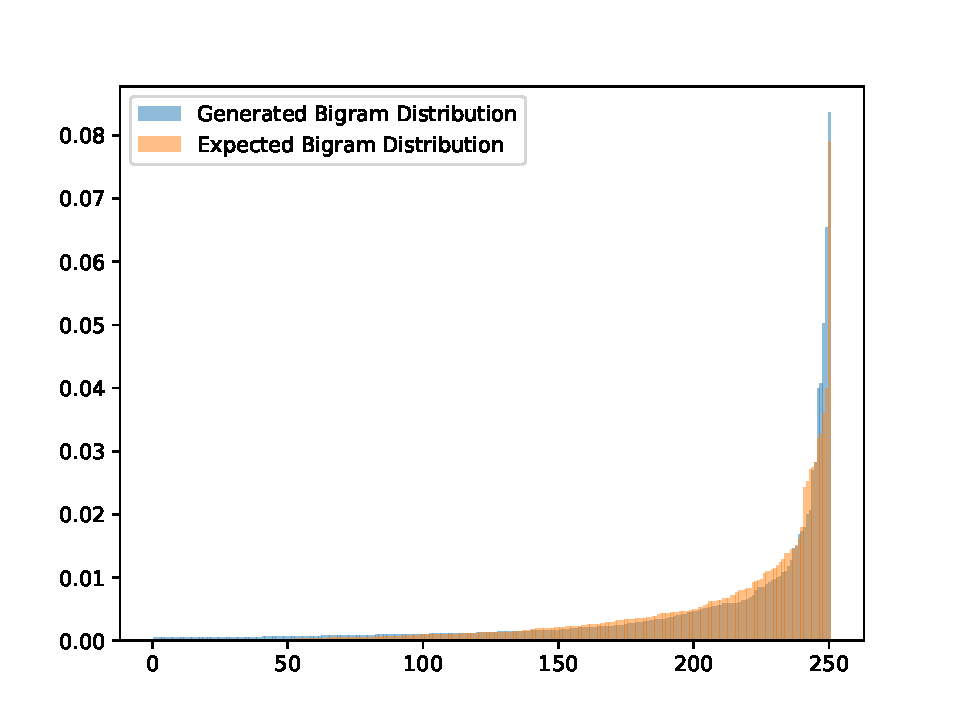
\includegraphics[width=\linewidth]{img/plots/reddit/bigram_distribution_comparison_step_2500000.pdf}
	\centering
	\small
	\text{Snapshot 2.5M}
	\endminipage\hfill
	\minipage{0.5\textwidth}
	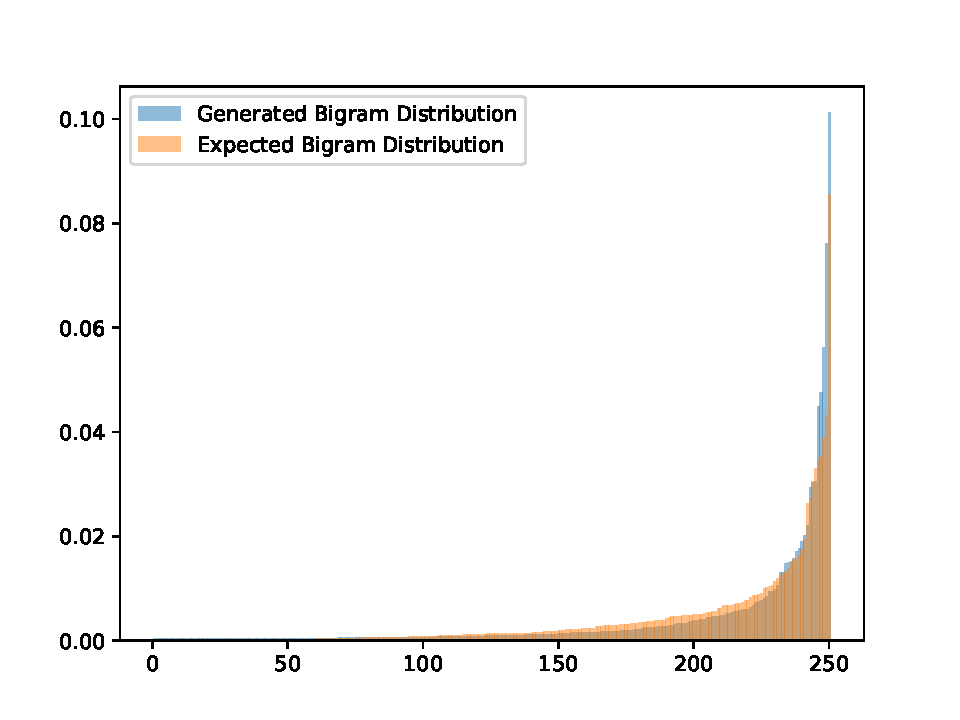
\includegraphics[width=\linewidth]{img/plots/reddit/bigram_distribution_comparison_step_3000000.pdf}
	\centering
	\small
	\text{Snapshot 3.0M}
	\endminipage\hfill
	\caption{Comparison of the distributions of the top 250 most used bi-grams for the responses of the Reddit model (orange) when using the test dataset and the distribution within the training dataset (blue). The distributions are compared for each snapshot available.}
	\label{results:bigram:distributions:reddit}
\end{figure}

\subsection{Language Diversity}
We now analyze the language diversity of the outputs produced by the two models over the different snapshots.  For this purpose, we are analyzing how large the share of the top 10 uni-, bi-gram and sentences within the entirety of the generated responses is when using the respective test datasets. The results can be seen in the Table~\ref{results:top_10_frequency:reddit} for Reddit and \ref{results:top_10_frequency:OpenSubtitles} for OpenSubtitles. 

In the Tables, three different categories are shown: Uni-grams, bi-grams and sentences. For each of these categories, we have summed up the occurrence frequencies of the top 10 most occurring instances for the respective category. These sums can be seen in the \emph{Top Count} columns. The columns named \emph{All Count} contain the total amount of all instances for each category per snapshot. The ratio of the \emph{Top Count} value compared to the \emph{All Count} value can be seen in the \emph{Top Freq.} column for each category and snapshot.
\todo{add more telling column names to the tables}

The first thing which is noticeable when comparing the values from the two Tables is that the Reddit outputs seem to be composed of much more uni- and bi-grams. This can be seen when comparing the \emph{Top Count} values from both Tables. This signifies that the outputs of the Reddit model are of greater length on average than the outputs of the OpenSubtitles model because the number of sentences stays the same for both. This might be one of the reasons why the results from the Sent2Vec analysis (see Chapter~\ref{results:performance_on_test_datasets}) are much better for the Reddit than the OpenSubtitles model.

At first, we tried to see a tendency on how language diversity develops when using the absolute values from the \emph{Top Count} columns, but we could not. This is the reason why we added the relative values from the \emph{Top Freq.} columns. The problem with using the absolute values is, that the number used uni- and bi-grams changes between the snapshots. However, when we start using the relative values we can compare the different snapshots to each other by means of diversity of the outputs. 

\begin{table}[H]
	\centering
	\begin{adjustbox}{max width=\textwidth}
		\begin{tabular}{llllllllll}
			\toprule
			& Words &&&Bi-Gramm&&&Sentences&&\\
			Snapshot & Top 10 Count & All Count& Top 10 freq. \%&  Top 10 Count& All Count& Top 10 freq. \%&  Top 10 Count& All Count& Top 10 freq. \%\\
			\midrule
			0.5M & 516,756	 & 1,035,956	& 49.88\%	&306,757	&1,033,319	&29.69\%	&102,770	&249,984	&41.11\%\\
			1.0M & 639,494	 & 860,951		& 74.28\%	&504,946	&858,145	&58.84\%	&188,748	&249,984	&75.50\%\\
			1.5M & 624,243	 & 1,249,230	& 49.97\%	&378,566	&1,233,467	&30.70\%	&108,312	&249,984	&43.33\%\\
			2.0M & 589,721	 & 814,101		& 72.44\%	&475,120	&807,087	&58.87\%	&181,585	&249,984	&72.64\%\\
			2.5M & 651,779	 & 1,131,640	& 57.60\%	&395,060	&1,117,436	&35.35\%	&92,273		&249,984	&36.91\%\\
			3.0M & 991,879	 & 1,470,695	& 40.10\%	&718,034	&1,459,490	&49.20\%	&105,245	&249,984	&42.10\%\\
			\bottomrule
		\end{tabular}
	\end{adjustbox}
	\caption{Top 10 uni-grams, bi-grams and sentences with summed up frequencies and computed share of the entirety of all instances for each category per OpenSubtitles snapshot.}
	\label{results:top_10_frequency:OpenSubtitles}
\end{table}
\todo{rework captions! Dirk: Es ist halt schon sehr kurz und bündig, aber eigentlich vollständig?}

\begin{table}[H]
	\centering
	\begin{adjustbox}{max width=\textwidth}
		\begin{tabular}{llllllllll}
			\toprule
			& Words &&&Bi-Gramm&&&Sentences&&\\
			Snapshot & Top 10 Count & All Count& Top 10 freq. \%&  Top 10 Count& All Count& Top 10 freq. \%&  Top 10 Count& All Count& Top 10 freq. \%\\
			\midrule
			0.5M & 2,712,157	 & 4,484,679	 & 60.48\%	&2,096,681	&4,483,620	&46.76\%	&86,408	&249,984	&34.57\%\\
			1.0M & 2,576,291	 & 4,294,209	 & 60.00\%	&1,941,620	&4,290,818	&45.25\%	&71,050	&249,984	&28.42\%\\
			1.5M & 1,918,226	 & 3,668,416	 & 52.29\%	&1,256,740	&3,663,402	&34.31\%	&46,590	&249,984	&18.64\%\\
			2.0M & 2,507,930	 & 4,577,892	 & 54.78\%	&1,665,799	&4,567,229	&36.47\%	&29,544	&249,984	&11.82\%\\
			2.5M & 1,623,645	 & 3,148,834	 & 51.56\%	&1,045,565	&3,134,900	&33.35\%	&73,475	&249,984	&29.39\%\\
			3.0M & 2,108,447	 & 3,614,679	 & 69.38\%	&1,449,193	&3,599,584	&40.26\%	&82,797	&249,984	&33.12\%\\
			\bottomrule
		\end{tabular}
	\end{adjustbox}
	\caption{Top 10 uni-grams, bi-grams and sentences with summed up frequencies and computed share of the entirety of all instances for each category per Reddit snapshot.}
	\label{results:top_10_frequency:reddit}
\end{table}
\todo{rework captions!}

We plot the \emph{Top Freq.} values for all the categories per model and snapshot to visualize the development of the values for the different categories and possible correlations between them. The resulting graphics can be seen in Figures~\ref{results:language_model:diversity:opensubtitles} and~\ref{results:language_model:diversity:reddit}. The plots can be interpreted that decreasing values imply that the share of the top 10 most occurring instances per category reduce compared to the whole number of instances of this category. We interpret this as an increase in language diversity, which is positive.

In the mentioned plots, we observe several peculiarities, which we are going to discuss per model below.

\paragraph{OpenSubtitles} The plot for the OpenSubtitles (see Figure~\ref{results:language_model:diversity:opensubtitles}) shows the same patterns as with the n-gram distributions seen before. Over the course of the training, it appears that the diversity of the language model wobbles up and down. Our assumption for this flattering development is similar as with the n-gram distributions:  Because this occurs only with the OpenSubtitles model and not with the Reddit, it is most probably related to the dataset. The causes could be the missing turn-taking information  as mentioned in the in \ref{data:preprocessing}, or the spoken language. But, if we take a close look at the numbers, we see that the peaks are getting smaller over time. For example, the share of the top 10 sentences and words for the 2.0M snapshot is about $2\%$ to $3\%$ lower than with the 1.0M model. The difference is, with $0.02\%$, much smaller for the bi-grams. Nevertheless, overall we can see a tendency that the model starts to use a more diverse language model the longer the training advances.

\begin{figure}[H]
	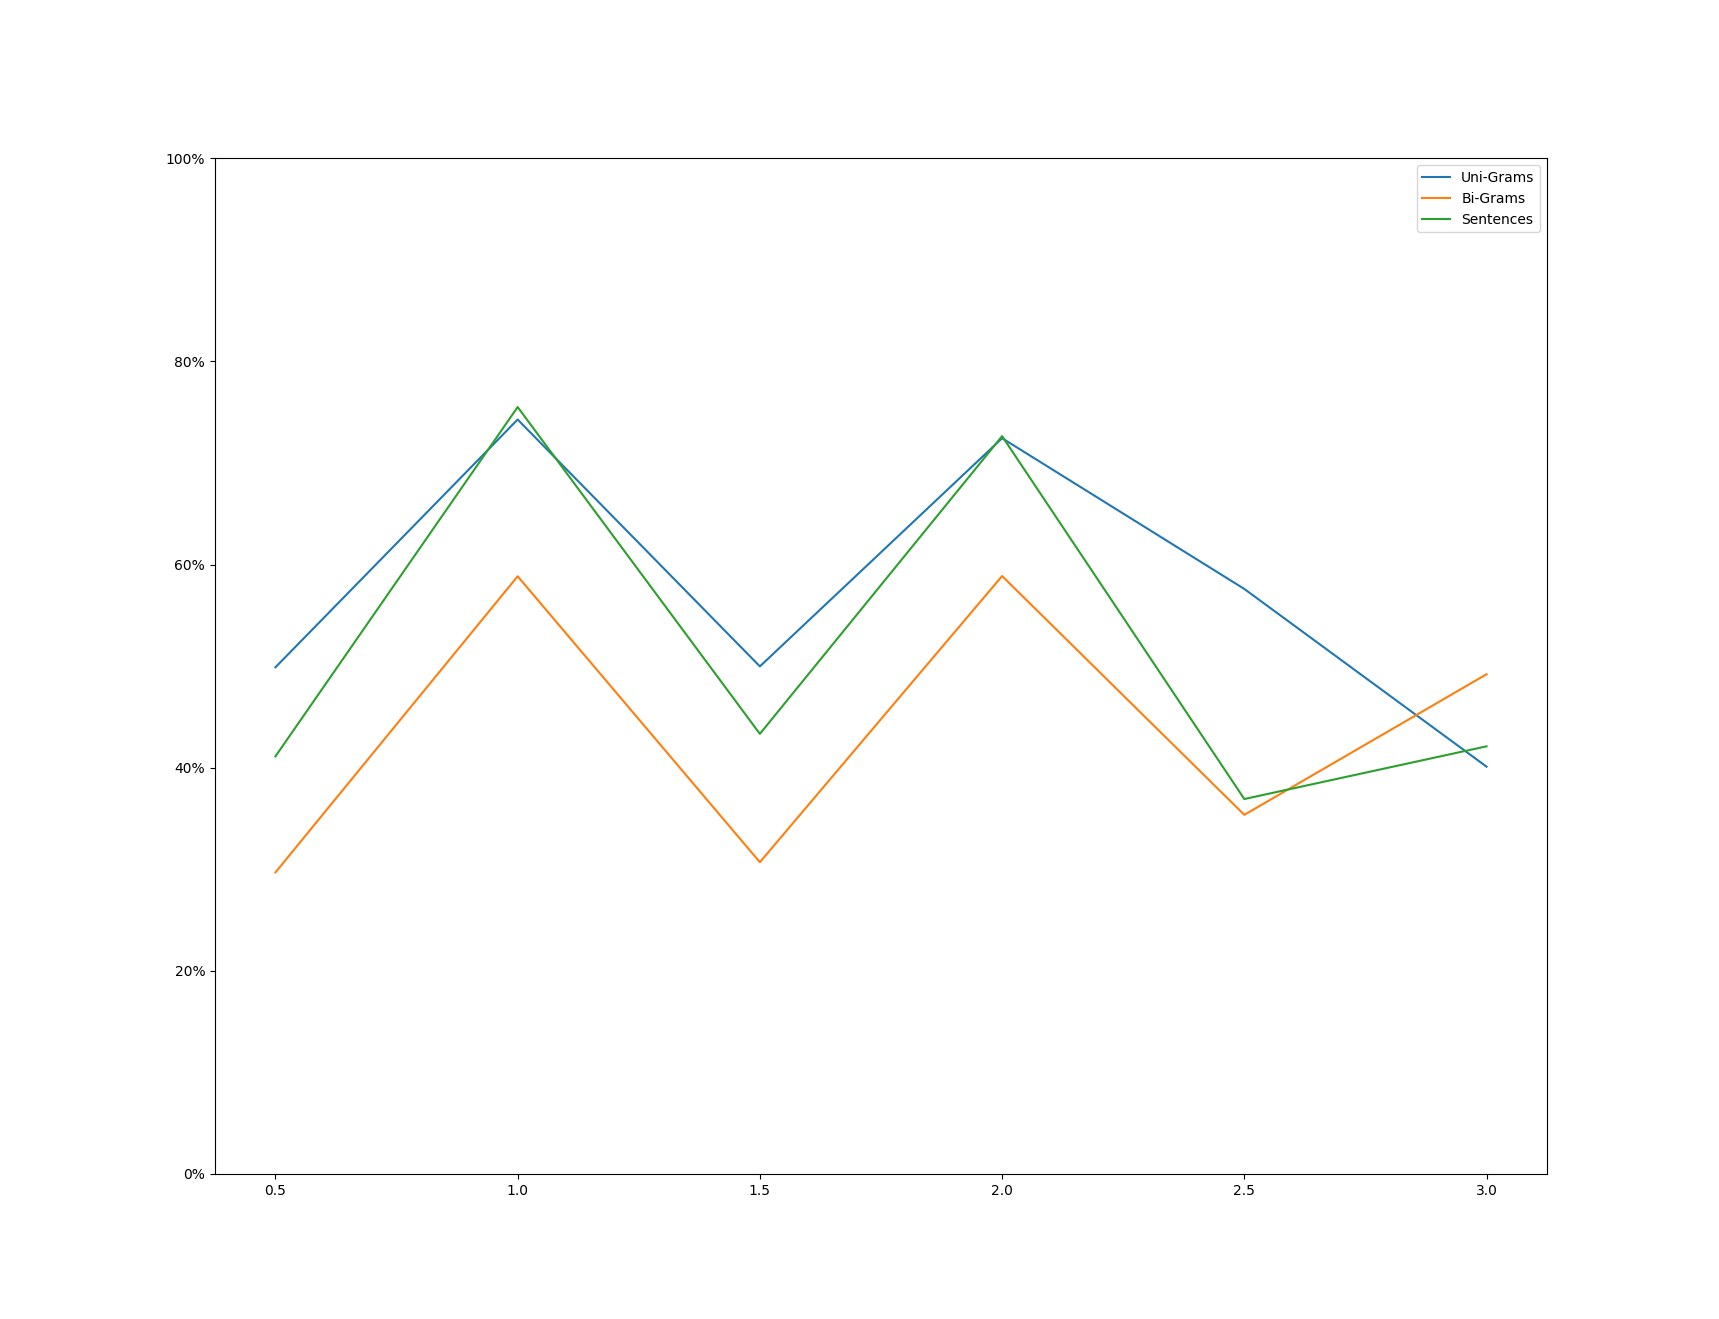
\includegraphics[width=\linewidth]{img/plots/opensubtitles_not_reversed/diversity_perc_plot.png}
	\caption{Development of all uni-, bi-grams and sentences, in percent, that are covered by the top 10 most used instances of each category for the OpenSubtitles model.}
	\label{results:language_model:diversity:opensubtitles}
\end{figure}

\paragraph{Reddit} The plot for the Reddit model (see Figure~\ref{results:language_model:diversity:reddit}) reveals that the language model becomes more diverse over the course of the training until the maximum diversity (minimum in the plot) is achieved when using the 2.0M snapshot. From this point onwards, diversity continuously decreases for the rest of the training. This coincides with our opinion, that the model is most optimal when using the 2.0M snapshot. We assume this problematic behavior is caused by the fact, that between the snapshots 1.5M and 2.0M training is within its second epoch. This could lead to an overfitting effect, which worsens the results and diversity of the language used by the model.

\begin{figure}[H]
	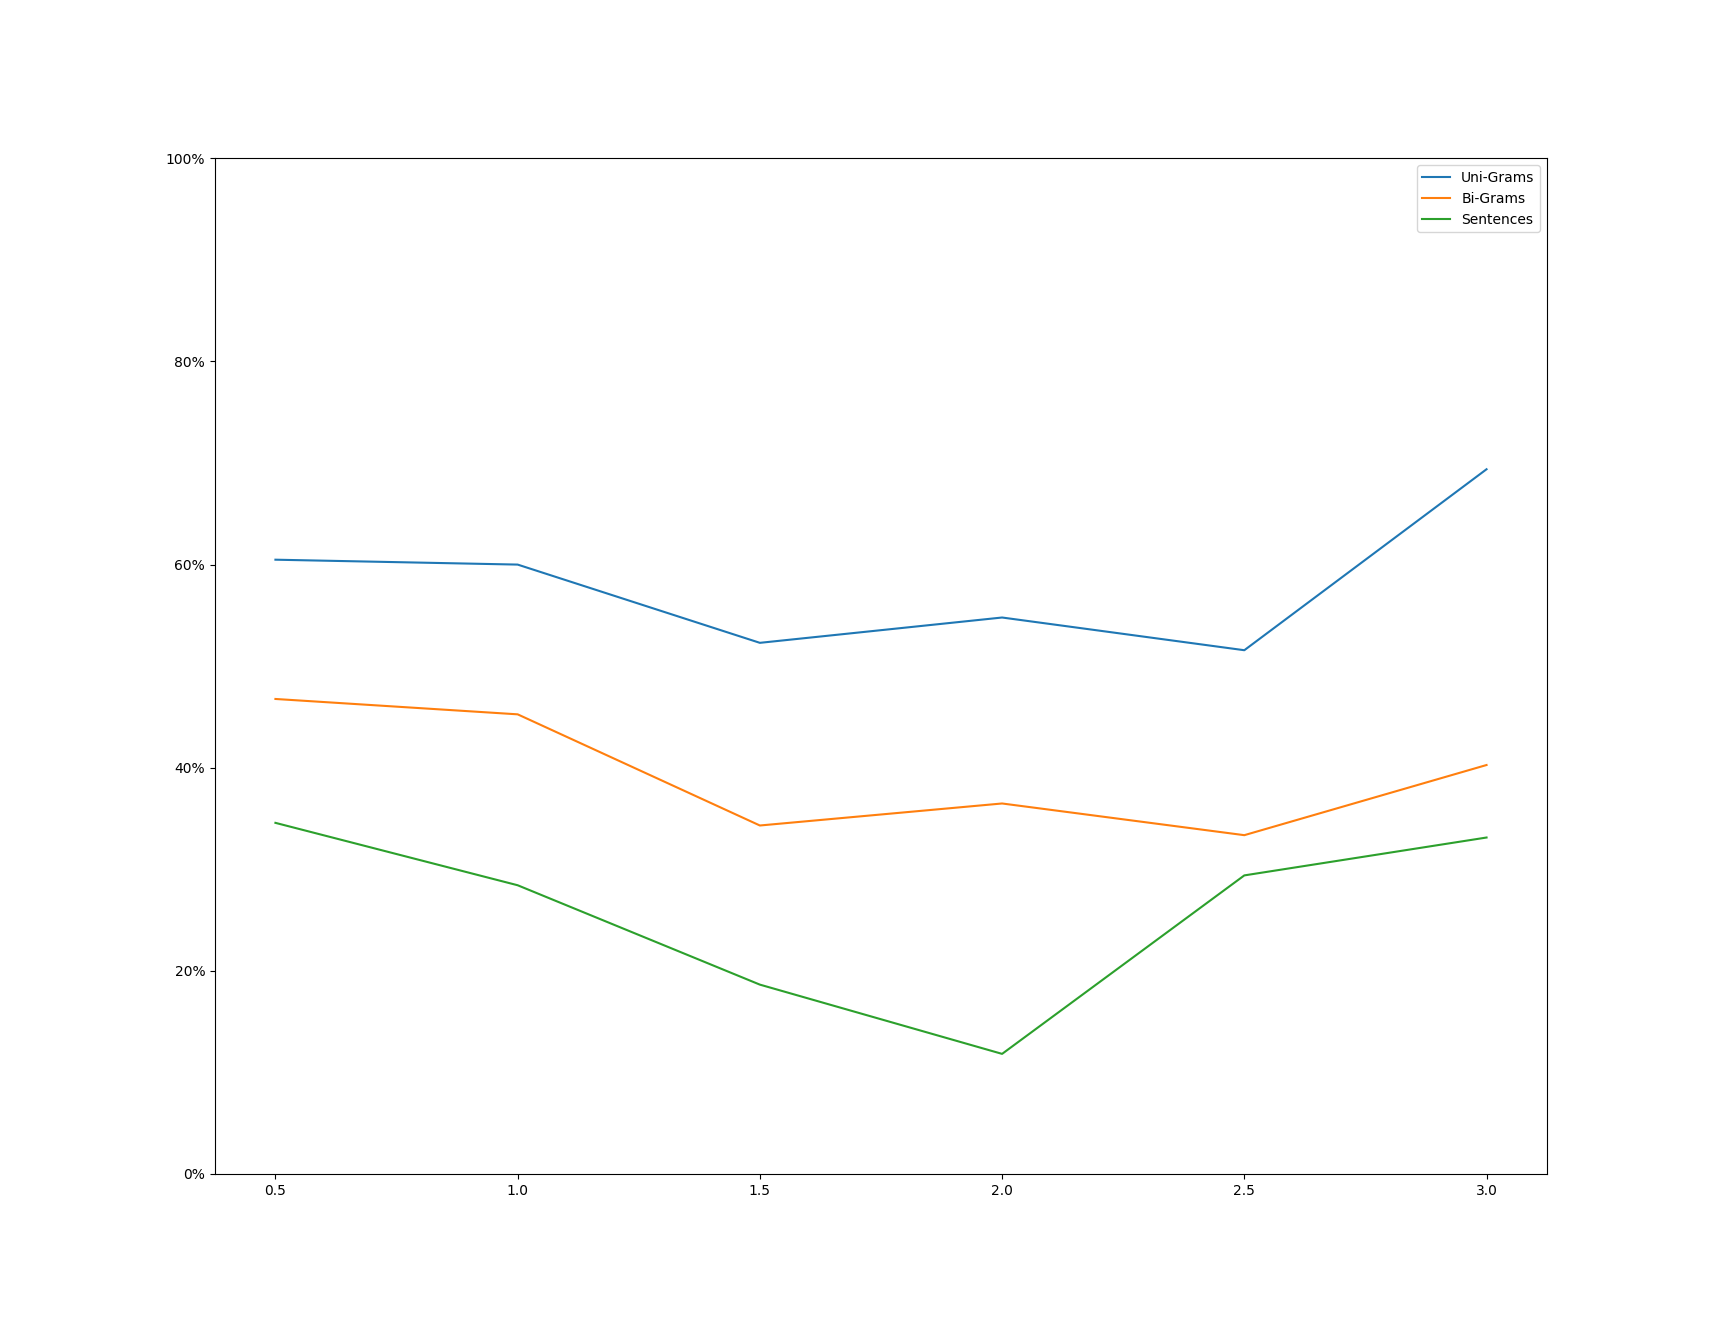
\includegraphics[width=\linewidth]{img/plots/reddit/diversity_perc_plot.png}
	\caption{Development of all uni-, bi-grams and sentences, in percent, that are covered by the top 10 most used instances of each category for the Reddit model.}
	\label{results:language_model:diversity:reddit}
\end{figure}

\subsection{Results}
Our analysis has shown that the distributions of uni- and bi-grams tend to fit the expected distributions better the longer the training advances. However, we found some interesting peculiarities we wanted to analyze with respect to language diversity.

This analysis has shown that the development of the language diversity is in direct relationship to the development of the mentioned n-gram distributions. We were also able to substantiate our subjective feeling, that the OpenSubtitles model improves over time, as the language diversity increase slowly. Additionally, we could also provide evidence that our opinion is correct that the Reddit model has the best performance when using the 1.5M or 2.0M snapshot as these two snapshots have indeed the greatest variety in the used language measured by our statistics. It does not allow us to completely explain the problem with generic responses, but we could show that the share of these generic responses tends to decrease with more training time.

Finally, the analysis showed that iterating over the same dataset multiple times is not recommended, as the Reddit model becomes worse after the snapshot 2.0M. This is particularly apparent when looking at the results of the 3.0M snapshot. Using a regularization technique, such as Dropout~\cite{Nitish:2014} would probably help when using a small dataset which is iterated multiple times.

With this, we conclude the quantitative analysis of the language model and start to do the human evaluation. This evaluation is conducted by comparing our model's results against results from others.

\section{Comparison with Other Models}
We now compare the results of our model with two others. As references we use: The CleverBot\footnote{http://www.cleverbot.com/} chatbot and the results from the paper ``Neural Conversational Model''~\cite{Vinyals:2015}, whose model architecture serves as the base of our model (see Chapter~\ref{methods:architecture}). We test the quality of the responses from our models if confronted with utterances of different types and difficulties. Our expectation is to reveal the strengths and weaknesses of our models.

\subsection{Cleverbot}
\label{results:comparison:cleverbot}
We start with the comparison with the CleverBot. CleverBot is a non-deterministic chatbot, meaning similar inputs can create different outputs if fed at different points in time. The responses listed below were generated at the June 1$^{\operatorname{st}}$ between 12:00 am and 03:00 pm.

\paragraph{Simple Utterance} We start by using the two simple utterances ``How are you?'' and ``Hi there, i m john!''. As one can see in the Tables~\ref{results:example1_output:OpenSubtitle_compared} and~\ref{results:example1_output:Reddit_compared}, our OpenSubtitles model as well as the CleverBot answered this question with satisfying response. The responses of the Reddit model to the utterance ``Hi there, i m john!'' are rather poor as none of them is really meaningful.
\\
\begin{table}[H]
	\centering
	\begin{adjustbox}{max width=\textwidth}
		\begin{tabularx}{\textwidth}{lX}
			\toprule
			Input: 	& \texttt{Hi, how are you?}\\
			\midrule
			0.5M: 	& \texttt{how are you ?}\\
			1.0M: 	& \texttt{i m fine}\\
			1.5M:	& \texttt{i m good}\\
			2.0M:	& \texttt{good}\\
			2.5M:	& \texttt{good}\\
			3.0M:	& \texttt{good}\\
			Cleverbot:	& \texttt{I'm good. How are you?}\\
			\bottomrule
		\end{tabularx}
	\end{adjustbox}
\caption{Responses from the OpenSubtitles model per snapshot compared to the CleverBot response. The input utterance is ``How are you?''.}
\label{results:example1_output:OpenSubtitle_compared}

\end{table}
\begin{table}[H]
	\centering
	\begin{adjustbox}{max width=\textwidth}
		\begin{tabularx}{\textwidth}{lX}
			\toprule
			Input: 	& \texttt{Hi there, i m john!}\\
			\midrule
			0.5M:	& \texttt{<unknown>}\\
			1.0M: 	& \texttt{i m not a fan of the <unknown> , but i m not sure if you re a <unknown> .}\\
			1.5M: 	& \texttt{i m not the only one who thought this was a good idea .}\\
			2.0M:	& \texttt{i m a <unknown> !}\\
			2.5M:	& \texttt{i m not your buddy , guy .}\\
			3.0M:	& \texttt{i m not .}\\
			Cleverbot:	& \texttt{So what are you doing?}\\
			\bottomrule
		\end{tabularx}
	\end{adjustbox}
	\caption{Responses from the Reddit model per snapshot compared to the CleverBot response. The input utterance is ``Hi there, i m john!''.}
	\label{results:example1_output:Reddit_compared}
\end{table}

\paragraph{Closed Question} In the next step we are comparing responses produced when using a closed question as the utterance. The results are documented in the Tables~\ref{results:example2_output:OpenSubtitle_compared} and~\ref{results:example2_output:Reddit_compared}. With this type of utterance, we intend to evaluate if the models understand a closed question and can respond appropriately.

Our models can respond to closed questions appropriately, as both of them provide useful answers. The CleverBot seems to have problems with this question, probably because it does not understand how the concepts of flying and birds are related.
\\
\begin{table}[H]
	\centering
	\begin{adjustbox}{max width=\textwidth}
		\begin{tabularx}{\textwidth}{lX}
			\toprule
			Input: 	& \texttt{Can birds fly?}\\
			\midrule
			0.5M: 	& \texttt{no}\\
			1.0M: 	& \texttt{i can t}\\
			1.5M:	& \texttt{yeah , but in the meantime , i can t swim}\\
			2.0M:	& \texttt{no}\\
			2.5M:	& \texttt{i can t}\\
			3.0M:	& \texttt{sure}\\
			Cleverbot:	& \texttt{Some say they can.}\\
			\bottomrule
		\end{tabularx}
	\end{adjustbox}
	\caption{Responses to a contextual question from the OpenSubtitles model per snapshot and the CleverBot response.}
	\label{results:example2_output:OpenSubtitle_compared}
\end{table}
\begin{table}[H]
	\centering
	\begin{adjustbox}{max width=\textwidth}
		\begin{tabularx}{\textwidth}{lX}
			\toprule
			Input: 	& \texttt{Can birds fly?}\\
			\midrule
			0.5M: 	& \texttt{i m not sure if this is a movie , but i m not sure if it s a movie .}\\
			1.0M: 	& \texttt{i can not imagine how much i can get this .}\\
			1.5M:	& \texttt{i m sure he s a <unknown> .}\\
			2.0M:	& \texttt{yes}\\
			2.5M:	& \texttt{yes}\\
			3.0M:	& \texttt{yes}\\
			Cleverbot:	& \texttt{Some say they can.}\\
			\bottomrule
		\end{tabularx}
	\end{adjustbox}
	\caption{Responses to a closed question from the Reddit model per snapshot and the CleverBot response.}
	\label{results:example2_output:Reddit_compared}
\end{table}

\paragraph{Knowledge Question}
The next kind of utterance are knowledge questions. With this kind of questions, we would like to evaluate if the models have general knowledge. The results can be seen in the Tables~\ref{results:example3_output:OpenSubtitle_compared} and~\ref{results:example3_output:Reddit_compared}.

The responses to the question about the color of the sky show an interesting development. Until the snapshot 2.0M, the responses were not appropriate and did not have any meaningful content\footnote{The response ``the jews'' comes from the fact, that in the beginning of the OpenSubtitles dataset, there are a lot of conversations related to movies about Nazism and world war II.}. However, from the snapshot 2.0M on the model answers in a correct way, even though it replies once with red as the answer, which can only be a correct answer in the morning and evening. If we expect blue as the answer, it is also correct twice, whereas the last response from the 3.0M seems to be the best. The answer of the CleverBot to this question is quite meaningless and is not related at all to the provided question.

The response to the question, where the Reddit model lives, was answered in a satisfying way, whereby the response of the 2.0M snapshot is worse than the previous models. It clearly understands the context of the question, as it always answers with a location-related answer. The CleverBot answers this question completely correct.

\begin{table}[H]
	\centering
	\begin{adjustbox}{max width=\textwidth}
		\begin{tabularx}{\textwidth}{lX}
			\toprule
			Input: 	& \texttt{What color is the sky?}\\
			\midrule
			0.5M: 	& \texttt{the jews}\\
			1.0M: 	& \texttt{it s a}\\
			1.5M:	& \texttt{oh , it s not}\\
			2.0M:	& \texttt{it s the blue}\\
			2.5M:	& \texttt{the red}\\
			3.0M:	& \texttt{blue}\\
			Cleverbot:&\texttt{*Kisses playfully*.}\\
			\bottomrule
		\end{tabularx}
	\end{adjustbox}
	\caption{Responses to a knowledge-related question with the OpenSubtitles model per snapshot and the CleverBot response.}
	\label{results:example3_output:OpenSubtitle_compared}
\end{table}
\begin{table}[H]
	\centering
	\begin{adjustbox}{max width=\textwidth}
		\begin{tabularx}{\textwidth}{lX}
			\toprule
			Input: 	& \texttt{In which country do you live?}\\
			\midrule
			0.5M: 	& \texttt{i m not sure if you re a <unknown> .}\\
			1.0M: 	& \texttt{i live in canada .}\\
			1.5M:	& \texttt{i live in the uk .}\\
			2.0M:	& \texttt{the country}\\
			2.5M:	& \texttt{canada}\\
			3.0M:	& \texttt{sweden}\\
			Cleverbot:&\texttt{The United States.}\\
			\bottomrule
		\end{tabularx}
	\end{adjustbox}
	\caption{Responses to a knowledge-related question from the Reddit model per snapshot and the CleverBot response.}
	\label{results:example3_output:Reddit_compared}
\end{table}

\paragraph{Contextual Question} 
With the next question, we want to evaluate if the models are capable of using contextual information to build an appropriate response. The results can be seen in the Tables~\ref{results:example4_output:OpenSubtitle_compared} and~\ref{results:example4_output:Reddit_compared}.

As visible below, the OpenSubtitles model has major issues with this kind of utterances, as all the responses are not fitting. The only response with certain usability is the one of the 2.5M model, where at least the correct color is included in the response. The response of the CleverBot is in this case also not of relevance.

The responses of the Reddit model are better fitting to the question, but they are also reasonably poor compared to our expectation. At least the model tries to formulate responses where the two colors of the question are included. The answer of the CleverBot is again useless. This time even less related to the question, compared to the response given by the OpenSubtitles model when using the question.
\\
\begin{table}[H]
	\centering
	\begin{adjustbox}{max width=\textwidth}
		\begin{tabularx}{\textwidth}{lX}
			\toprule
			Input: 	& \texttt{I wear a blue jeans. What color do my jeans have?}\\
			\midrule
			0.5M: 	& \texttt{<unknown> <unknown>}\\
			1.0M: 	& \texttt{i don t know}\\
			1.5M:	& \texttt{oh , yeah}\\
			2.0M:	& \texttt{i m not a prostitute}\\
			2.5M:	& \texttt{i got a blue blue}\\
			3.0M:	& \texttt{i m not a fan}\\
			Cleverbot:	& \texttt{You don't have any.}\\
			\bottomrule
		\end{tabularx}
	\end{adjustbox}
	\caption{Responses to a contextual question from the OpenSubtitles model per snapshot and the CleverBot response.}
	\label{results:example4_output:OpenSubtitle_compared}
\end{table}
\begin{table}[H]
	\centering
	\begin{adjustbox}{max width=\textwidth}
		\begin{tabularx}{\textwidth}{lX}
			\toprule
			Input: 	& \texttt{I wear a red pullover and blue jeans. What color do my jeans have?}\\
			\midrule
			0.5M: 	& \texttt{i m a big fan of the <unknown> .}\\
			1.0M: 	& \texttt{i m not a fan of the <unknown> , but i do nt know what you re talking about .}\\
			1.5M:	& \texttt{i m a white male and i wear pants .}\\
			2.0M:	& \texttt{i wear a red shirt and i wear glasses .}\\
			2.5M:	& \texttt{i m a red blue and blue blue .}\\
			3.0M:	& \texttt{i m a white male and i have a blue blue shirt .}\\
			Cleverbot:	& \texttt{What is your opinion on President Obama. And don't ask me mine without saying yours first!.}\\
			\bottomrule
		\end{tabularx}
	\end{adjustbox}
	\caption{Responses to a contextual question from the Reddit model per snapshot and the CleverBot response.}
	\label{results:example4_output:Reddit_compared}
\end{table}

\paragraph{Specific Question}
The next questions are more specific. We are going to ask the OpenSubtitles model a simple mathematical question and the Reddit models a question about the TV series ``Game of Thrones''. The results can be seen in the Tables~\ref{results:example5_output:OpenSubtitle_compared} and~\ref{results:example5_output:Reddit_compared}.

The responses of the OpenSubtitles model are quite clear in the beginning: it does not know the answer or does not understand the question at all. However, the later snapshots (i.e. from 2.0M onwards), it seems to understand that it has to answer with a number. Sadly, the correct result is not included in the generated responses. The CleverBot also does not understand how to answer such a question.

The Reddit model has an interesting twist in its responses. In the beginning, it starts by responding with generic responses which do not seem to have any relation to the TV series. However, the funny response\footnote{``Hodor'' is a character in the ``Game of Thrones'' series who is only capable of saying its own name. In case of danger he starts yelling its name over and over again, which occurs several times throughout the series.} at the end (i.e. ``hodor, hodor, ...'') indicates that it understands the question at least to some degree, even though the response does not contain any actual information about the series. The CleverBot response is a mystery to us, as we could not find any character or other scene in the series where a ``Dani'' is mentioned.
\\
\begin{table}[H]
	\centering
	\begin{adjustbox}{max width=\textwidth}
		\begin{tabularx}{\textwidth}{lX}
			\toprule
			Input: 	& \texttt{How much is 1 added to 2?}\\
			\midrule
			0.5M: 	& \texttt{i don t know}\\
			1.0M: 	& \texttt{i don t know}\\
			1.5M:	& \texttt{i don t know}\\
			2.0M:	& \texttt{ten dollars}\\
			2.5M:	& \texttt{50}\\
			3.0M:	& \texttt{2}\\
			Cleverbot:	& \texttt{I don't know.}\\
			\bottomrule
		\end{tabularx}
	\end{adjustbox}
	\caption{Responses to a mathematical question from the OpenSubtitles model per snapshot and the CleverBot response.}
	\label{results:example5_output:OpenSubtitle_compared}
\end{table}
\begin{table}[H]
	\centering
	\begin{adjustbox}{max width=\textwidth}
		\begin{tabularx}{\textwidth}{lX}
			\toprule
			Input: 	& \texttt{Can you tell me something about game of thrones?}\\
			\midrule
			0.5M: 	& \texttt{i m not sure if you re a fan of the movie , but i m not sure if you re going to be}\\
			& \texttt{a fan of the}\\
			1.0M: 	& \texttt{i m not sure what you re saying .}\\
			1.5M:	& \texttt{i m not sure if i m going to be watching this .}\\
			2.0M:	& \texttt{i m not sure if you re joking , but i m pretty sure that s the case .}\\
			2.5M:	& \texttt{i m not sure if you re talking about the game or the game , but i think the game}\\
			& \texttt{is a little different .}\\
			3.0M:	& \texttt{hodor hodor hodor hodor hodor hodor hodor hodor hodor hodor hodor hodor hodor hodor }\\
			& \texttt{hodor hodor hodor hodor hodor hodor hodor hodor hodor hodor hodor hodor hodor hodor}\\
			Cleverbot:	& \texttt{Dani is life.}\\
			\bottomrule
		\end{tabularx}
	\end{adjustbox}
	\caption{Responses to a question about a TV series from the Reddit model per snapshot and the CleverBot response.}
	\label{results:example5_output:Reddit_compared}
\end{table}

\paragraph{Answers to Statements}
Until now, we have only asked questions to our models. We would now like to see how the responses to statements instead of questions are. The results can be seen in the Tables~\ref{results:example6_output:OpenSubtitle_compared} and~\ref{results:example6_output:Reddit_compared}.

The responses of the OpenSubtitles model are useful from the snapshot 1.5M onward. Especially the answer for the snapshot 2.0M is interesting, as this seems to indicate that the model has some kind of empathy for the other person in the dialog, expressed in the response ``i m sorry''. The response of the CleverBot signifies that it understands the statement to some degree, but does not know what to answer.

The responses of the Reddit model to the statement that it has a bad opinion are rather poor across all snapshots, with the response from the 1.5M model being the only one which is remotely useful. The response of the CleverBot is a pretty speedy answer in this case.
\\
\begin{table}[H]
	\centering
	\begin{adjustbox}{max width=\textwidth}
		\begin{tabularx}{\textwidth}{lX}
			\toprule
			Input: 	& \texttt{i invited her to a public reading of my work , but she never came .}\\
			\midrule
			0.5M: 	& \texttt{she was a}\\
			1.0M: 	& \texttt{i don t know}\\
			1.5M:	& \texttt{really ?}\\
			2.0M:	& \texttt{i m sorry}\\
			2.5M:	& \texttt{she s been in a lot of trouble}\\
			3.0M:	& \texttt{she s not a fan}\\
			Cleverbot:	& \texttt{Who?}\\
			\bottomrule
		\end{tabularx}
	\end{adjustbox}
	\caption{Responses to a statement from the OpenSubtitles model per snapshot and the CleverBot response.}
	\label{results:example6_output:OpenSubtitle_compared}
\end{table}
\begin{table}[H]
	\centering
	\begin{adjustbox}{max width=\textwidth}
		\begin{tabularx}{\textwidth}{lX}
			\toprule
			Input: 	& \texttt{Your film taste is bad and your opinion does not interest me!}\\
			\midrule
			0.5M: 	& \texttt{i m not sure what you re saying .}\\
			1.0M: 	& \texttt{i m not your friend , but i m not a fan of the <unknown> .}\\
			1.5M:	& \texttt{i m sorry , i did nt know that .}\\
			2.0M:	& \texttt{i m not a fan of the movie , but i m not sure if you re going to be a fan of the film .}\\
			2.5M:	& \texttt{i m not a fan of the film , but i think it s a good movie .}\\
			3.0M:	& \texttt{i m not sure if you re being sarcastic or not .}\\
			Cleverbot:	& \texttt{And for me your opinion does not matter.}\\
			\bottomrule
		\end{tabularx}
	\end{adjustbox}
	\caption{Responses to a statement from the Reddit model per snapshot and the CleverBot response.}
	\label{results:example6_output:Reddit_compared}
\end{table}

\paragraph{Self-Concept} Finally, we have an interesting answer from the Reddit model to the question ``What are you?''. The responses can be seen in Table~\ref{results:example7_output:Reddit_compared}. All snapshots produce bad responses, apart from the last, where it answered that it is a bot. This is an interesting answer because it shows that the model seems to potentially have some kind of self-concept. We cannot explain that, as the model was trained on comments from Reddit discussion about movies and series. Nevertheless, it is an interesting answer to see.

\begin{table}[H]
	\centering
	\begin{adjustbox}{max width=\textwidth}
		\begin{tabularx}{\textwidth}{lX}
			\toprule
			Input: 	& \texttt{What are you?}\\
			\midrule
			0.5M: 	& \texttt{i m not a fan of the movie , but i m a huge fan of the movie .}\\
			1.0M: 	& \texttt{i m not a fan of the <unknown> , but i m not a fan of the <unknown> .}\\
			1.5M:	& \texttt{i m not .}\\
			2.0M:	& \texttt{i m not .}\\
			2.5M:	& \texttt{i m not .}\\
			3.0M:	& \texttt{i m a bot .}\\
			Cleverbot:	& \texttt{A human, what are you??}\\
			\bottomrule
		\end{tabularx}
	\end{adjustbox}
	\caption{Responses to a self-concept question from the Reddit models and the CleverBot response.}
	\label{results:example7_output:Reddit_compared}
\end{table}

Sadly, we were not able to find a similar response when using the OpenSubtitles model.

\subsection{Neural Conversational Model}
\label{results:comparison:ncm}
In this Section, we are going to compare the results from the paper ``Neural Conversation Model'' (NCM) with the resulting responses from our models. To compare the responses, we are going to use utterances from the paper and show all the responses from all OpenSubtitles snapshots, but only the (subjectively) best response from the Reddit model, as the NCM model was trained on the OpenSubtitles dataset. The responses can be seen in the Tables~\ref{results:example8_output:Neural_Conversational_Model_compared} to~\ref{results:example14_output:Neural_Conversational_Model_compared}. The categories where the input utterances came from in the paper are noted in the Table descriptions. A discussion of the results can be found at the end of this Chapter.

In this Section, we do not provide individual evaluations to the model responses, as the objective was to gain an overall impression of the quality of responses to individual utterances.

We are only showing a part of the dialogs which were evaluated. All other can be found in Appendix~\ref{apendix:results:compared_with_NCM}.
\\
\begin{table}[H]
	\centering
	\begin{adjustbox}{max width=\textwidth}
		\begin{tabularx}{\textwidth}{lX}
			\toprule
			Input: 	& \texttt{what year were you born ?}\\
			\midrule
			\emph{OpenSubtitles}\\
			0.5M: 	& \texttt{a lot of people}\\
			1.0M: 	& \texttt{i was a}\\
			1.5M:	& \texttt{a little}\\
			2.0M:	& \texttt{i was born}\\
			2.5M:	& \texttt{i don t know}\\
			3.0M:	& \texttt{i don t know}\\
			\midrule
			\emph{Reddit}\\
			2.0M:	& \texttt{i was born in the 90s .}\\
			\midrule
			\emph{NCM}:	& \texttt{1977 .}\\
			\bottomrule
		\end{tabularx}
	\end{adjustbox}
	\caption{Comparison between the NCM model and our OpenSubtitles model when using the utterance ``what year were you born ?'' from the ``Basic''.}
	\label{results:example8_output:Neural_Conversational_Model_compared}
\end{table}

\begin{table}[H]
	\centering
	\begin{adjustbox}{max width=\textwidth}
		\begin{tabularx}{\textwidth}{lX}
			\toprule
			Input: 	& \texttt{why are we here ?}\\
			\midrule
			\emph{OpenSubtitles}\\
			0.5M: 	& \texttt{because we were here}\\
			1.0M: 	& \texttt{i don t know}\\
			1.5M:	& \texttt{i don t know}\\
			2.0M:	& \texttt{i m sorry}\\
			2.5M:	& \texttt{we re here}\\
			3.0M:	& \texttt{we re here}\\
			\midrule
			\emph{Reddit}\\
			1.5M:	& \texttt{because we are nt .}\\
			\midrule
			\emph{NCM}:	& \texttt{i ’m not sure .}\\
			\bottomrule
		\end{tabularx}
	\end{adjustbox}
	\caption{Comparison between the NCM model and our OpenSubtitles model when using the utterance ``why are we here ?'' from the ``Basic'' category.}
	\label{results:example9_output:Neural_Conversational_Model_compared}
\end{table}
\begin{table}[H]
	\centering
	\begin{adjustbox}{max width=\textwidth}
		\begin{tabularx}{\textwidth}{lX}
			\toprule
			Input: 	& \texttt{are you a leader or a follower ?}\\
			\midrule
			\emph{OpenSubtitles}\\
			0.5M: 	& \texttt{no}\\
			1.0M: 	& \texttt{i m not a}\\
			1.5M:	& \texttt{i m sorry}\\
			2.0M:	& \texttt{i m not a prostitute}\\
			2.5M:	& \texttt{i m a}\\
			3.0M:	& \texttt{i m a}\\
			\midrule
			\emph{Reddit}\\
			2.0M:	& \texttt{i m a cyborg .}\\
			\midrule
			\emph{NCM}:	& \texttt{i'm a leader .}\\
			\bottomrule
		\end{tabularx}
	\end{adjustbox}
	\caption{Comparison between the NCM model and our OpenSubtitles model when using the utterance ``are you a leader or a follower ?'' from the ``General Knowledge Q\&A'' category.}
	\label{results:example10_output:Neural_Conversational_Model_compared}
\end{table}
\begin{table}[H]
	\centering
	\begin{adjustbox}{max width=\textwidth}
		\begin{tabularx}{\textwidth}{lX}
			\toprule
			Input: 	& \texttt{how much is ten minus two ?}\\
			\midrule
			\emph{OpenSubtitles}\\
			0.5M: 	& \texttt{four}\\
			1.0M: 	& \texttt{ten}\\
			1.5M:	& \texttt{two , two , three}\\
			2.0M:	& \texttt{ten dollars}\\
			2.5M:	& \texttt{ten}\\
			3.0M:	& \texttt{ten}\\
			\midrule
			\emph{Reddit}\\
			2.0M:	& \texttt{i m not sure how much i m going to get downvoted to hell .}\\
			\midrule
			\emph{NCM}:	& \texttt{seventy - two .}\\
			\bottomrule
		\end{tabularx}
	\end{adjustbox}
	\caption{Comparison between the NCM model and our OpenSubtitles model when using the utterance ``how much is ten minus two ?'' from the ``General Knowledge Q\&A'' category.}
	\label{results:example11_output:Neural_Conversational_Model_compared}
\end{table}
\begin{table}[H]
	\centering
	\begin{adjustbox}{max width=\textwidth}
		\begin{tabularx}{\textwidth}{lX}
			\toprule
			Input: 	& \texttt{what is the color of a yellow car ?}\\
			\midrule
			\emph{OpenSubtitles}\\
			0.5M: 	& \texttt{a <unknown> ?}\\
			1.0M: 	& \texttt{it s a}\\
			1.5M:	& \texttt{what ?}\\
			2.0M:	& \texttt{it s a blue blue}\\
			2.5M:	& \texttt{it s a blue}\\
			3.0M:	& \texttt{it s a yellow}\\
			\midrule
			\emph{Reddit}\\
			2.5M:	& \texttt{the yellow yellow yellow yellow yellow yellow yellow yellow yellow yellow yellow yellow yellow yellow yellow yellow yellow yellow yellow yellow yellow yellow yellow yellow yellow yellow yellow}\\
					\midrule
			\emph{NCM}:	& \texttt{yellow .}\\
			\bottomrule
		\end{tabularx}
	\end{adjustbox}
	\caption{Comparison between the NCM model and our OpenSubtitles model when using the utterance ``what is the color of a yellow car ?'' from the ``General Knowledge Q\&A'' category.}
	\label{results:example12_output:Neural_Conversational_Model_compared}
\end{table}
\begin{table}[H]
	\centering
	\begin{adjustbox}{max width=\textwidth}
		\begin{tabularx}{\textwidth}{lX}
			\toprule
			Input: 	& \texttt{what is the purpose of existence ?}\\
			\midrule
			\emph{OpenSubtitles}\\
			0.5M: 	& \texttt{the jews}\\
			1.0M: 	& \texttt{i don t know}\\
			1.5M:	& \texttt{you re just a fucking boy , man}\\
			2.0M:	& \texttt{i don t know}\\
			2.5M:	& \texttt{i m sorry}\\
			3.0M:	& \texttt{i m not sure}\\
			\midrule
			\emph{Reddit}\\
			1.5M:	& \texttt{i m not sure if you re joking or not , but i m sure you re }\\
			& \texttt{not familiar with the word .}\\
			\midrule
			\emph{NCM}:	& \texttt{to find out what happens when we get to the planet earth .}\\
			\bottomrule
		\end{tabularx}
	\end{adjustbox}
	\caption{Comparison between the NCM model and our OpenSubtitles model when using the utterance ``what is the purpose of existence ?'' from the ``Philosophical Q\&A'' category.}
	\label{results:example13_output:Neural_Conversational_Model_compared}
\end{table}

\begin{table}[H]
	\centering
	\begin{adjustbox}{max width=\textwidth}
		\begin{tabularx}{\textwidth}{lX}
			\toprule
			Input: 	& \texttt{what is the purpose of being intelligent?}\\
			\midrule
			\emph{OpenSubtitles}\\
			0.5M: 	& \texttt{the jews}\\
			1.0M: 	& \texttt{i don t know}\\
			1.5M:	& \texttt{i don t know}\\
			2.0M:	& \texttt{i don t know}\\
			2.5M:	& \texttt{i don t know}\\
			3.0M:	& \texttt{i don t know}\\
			\midrule
			\emph{NCM}:	& \texttt{to find out what it is .}\\
			\bottomrule
		\end{tabularx}
	\end{adjustbox}
	\caption{Comparison between the NCM model and our OpenSubtitles model when using the utterance ``what is the purpose of being intelligent?'' from the ``Philosophical Q\&A'' category.}
	\label{results:example20_output:OpenSubtitle}
\end{table}


\begin{table}[H]
	\centering
	\begin{adjustbox}{max width=\textwidth}
		\begin{tabularx}{\textwidth}{lX}
			\toprule
			Input: 	& \texttt{what are the things that i do to be immoral?}\\
			\midrule
			\emph{OpenSubtitles}\\
			0.5M: 	& \texttt{i don t know}\\
			1.0M: 	& \texttt{i don t know}\\
			1.5M:	& \texttt{what s the big idea ?}\\
			2.0M:	& \texttt{i don t know}\\
			2.5M:	& \texttt{i m a}\\
			3.0M:	& \texttt{i m not a criminal}\\
			\midrule
			\emph{Reddit}\\
			2.5M:	& \texttt{i think you re missing the point .}\\
			& \texttt{i don ’t know .}\\
			\midrule
			\emph{NCM}:	& \texttt{to find out what happens when we get to the planet earth .}\\
			\bottomrule
		\end{tabularx}
	\end{adjustbox}
	\caption{Comparison between the NCM model and our OpenSubtitles model when using the utterance ``what are the things that i do to be immoral?'' from the ``Morality'' category.}
	\label{results:example14_output:Neural_Conversational_Model_compared}
\end{table}

\subsection{Results}
In conclusion, our model is not as poor as expected by looking at the problems with the metrics and the generic responses caused by an undiversified language model.

In comparison to the CleverBot, our model provided several responses which were clearly superior in quality. But there were also cases where the CleverBot outperformed our model. This is probably related to the fact that the CleverBot works by fuzzily searching already witnessed conversations. This means, that if a conversation about a certain topic does not exist, the CleverBot has no facilities to create a meaningful answer. In contrast, our model instead has the ability to ``understand'' what is said and, hence can at least try to answer. Such an example would be the mathematical question ``How much is 1 added to 2?'', where the CleverBot simply answered ``I don't know'' and our model started to respond with numbers, even though the result was incorrect.

When comparing our models to the NCM model, one main issue of the model quickly becomes visible: The size of the model. For easily understandable utterances, the responses of our models are almost or as good as the responses from the NCM model. But if the utterances become more complicated, especially when it comes to philosophical or morality questions, our model starts to respond worse than the NCM model. This is, as said, not a real surprise, because our model is only half the size of the NCM model. Nevertheless, we conclude that our model is not superior, but in some regards of comparable quality as the NCM model.

\section{Beam-Search}
\label{results:beam_search}
There are always some poor responses shown in the previous Chapter. We would like to use our beam-search implementation as described in Chapter~\ref{fundamentals:decoding_approaches} to evaluate if this can help to increase response quality. We will evaluate this for three different examples, and evaluate if the responses generated by the beam-search decoder are superior to the responses of the greedy decoder. The evaluation was performed subjectively as usually the best answer does not necessarily correlate with the resulting log-probability score. This analysis is exemplarily done with the OpenSubtitles 3.0M model and a beam-width of $200$.

We only list the subjectively best responses here. All other responses can be found in Appendix~\ref{apendix:results:Beam-search-200:OpenSubtitle}. This has to do with the fact, that the subjectively best answer is usually not the best answer found when looking at the log-probability scores.

\paragraph{``what year were you born?''} The responses of the greedy decoder to this question can be found in the Table~\ref{results:example8_output:Neural_Conversational_Model_compared}. The original answers of the OpenSubtitles model were all reasonably poor, and it seemed that the model did not fully understand the question.

However, when using the beam-search decoder, there are several useful responses, such as ``1991'', ``last year'' or ``five years ago''. These responses are much better than the results initially generated by the greedy decoder. However, none of them is the highest ranked response and, hence is not returned by the model as the answer of choice. We provide a possible explanation for this anomaly later.

\paragraph{``i wear a blue jeans. what color do my jeans have?''} The second question was also answered pretty poorly initially. The results of the greedy decoder can be found in Table~\ref{results:example4_output:OpenSubtitle_compared}. The best response was delivered by the 2.5M model and was ``i got a blue blue'', which, at least, contains the searched color.

When using beam-search, better responses can be found. Such responses include ``blue'' and ``you know that''.

\paragraph{``what is the purpose of being intelligent?''} Finally, we wanted to explore a more complicated question from the moral Section of the NCM paper with beam-search. The responses of the greedy decoder can be found in Table~\ref{results:example20_output:OpenSubtitle}. All responses are of inferior quality and only consist of generic responses, such as ``i don t know''.

When using beam-search, several interesting responses were produced, fitting for such a philosophical question, such as ``well, it s complicated'', ``you can t know'' and ``well , it s nothing.''

\paragraph{Beam-Search Helps} The responses become much more diverse when using the beam-search decoder. The key problem is to choose the best response from the 200 generated responses. Per algorithm, the sum of the logarithmic probabilities at each step in the beam is used. However, this mechanism does not provide the answers we subjectively selected as ``best'' from the list. We are not quite sure if this is a problem related to the fact that the decoder was trained in a greedy fashion, but response generation was augmented with beam search, which might not be fully compatible. The implementation of beam-search was validated and is correct, as when beam-size is set to 1, answers are the same as when using the greedy decoder. Nevertheless, the implementation provided us insight into the inner mechanics of the model and we were able to find better responses than with the greedy decoder, even though such had to be selected from the list of responses manually.

\section{Thought Vectors for Input Sequences}\label{results:thought_vector_clustering} After the encoder has processed the entire input sequences, it forwards the thought vector to the decoder to construct the output sequence (see Chapter~\ref{fundamentals:seq2seq}). As this is the only direct connection of the encoder to the decoder, the encoder must ``encode'' all information into this thought vector. Hence, the thought vector hence represents an embedding of an input sequence in an $n$ dimensional vector space, where $n$ stands for the size of the thought vector. If we project the vectors into two dimensions via PCA, sentences with similar meanings should be clustered. That would substantiate that the models have a semantic understanding of the contents of these sentences.

To analyze the embeddings, we collect them for 15 different sample sentences and create respective thought vectors. We do this with both models and project the vectors via PCA into two-dimensional space. The results of this projection can be seen in Figure~\ref{results:thougth_vectors:embeddings:opensubtitles} and~\ref{results:thougth_vectors:embeddings:reddit} below.

\begin{figure}[!htb]
	\centering
	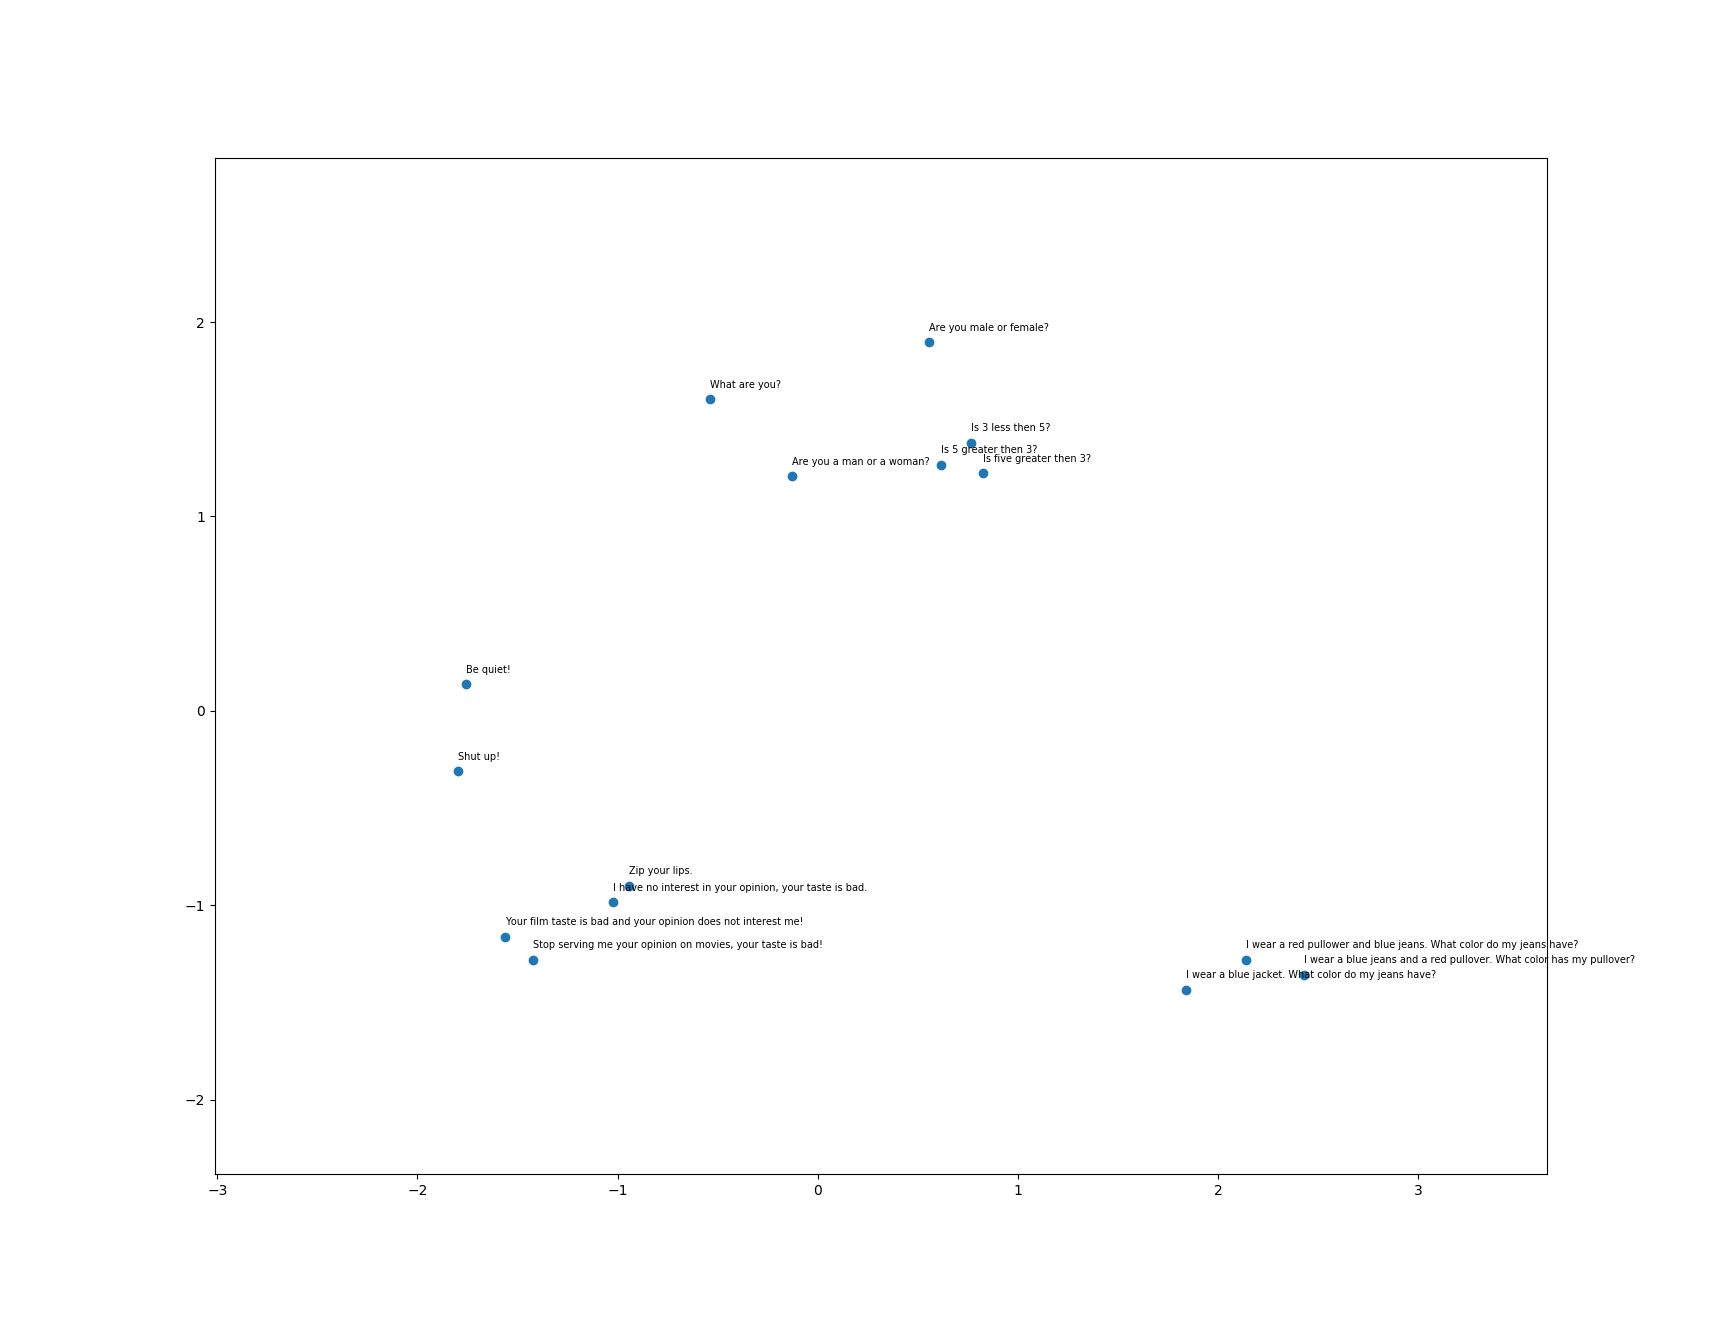
\includegraphics[width=14cm]{img/opensubtitles_thought_vector_embeddings.png}
	\caption{The projected thought vectors for 15 different sentences when using the OpenSubtitles 3.0M model. PCA was used for the projection.}
	\label{results:thougth_vectors:embeddings:opensubtitles}
\end{figure}

\begin{figure}[h]
	\centering
	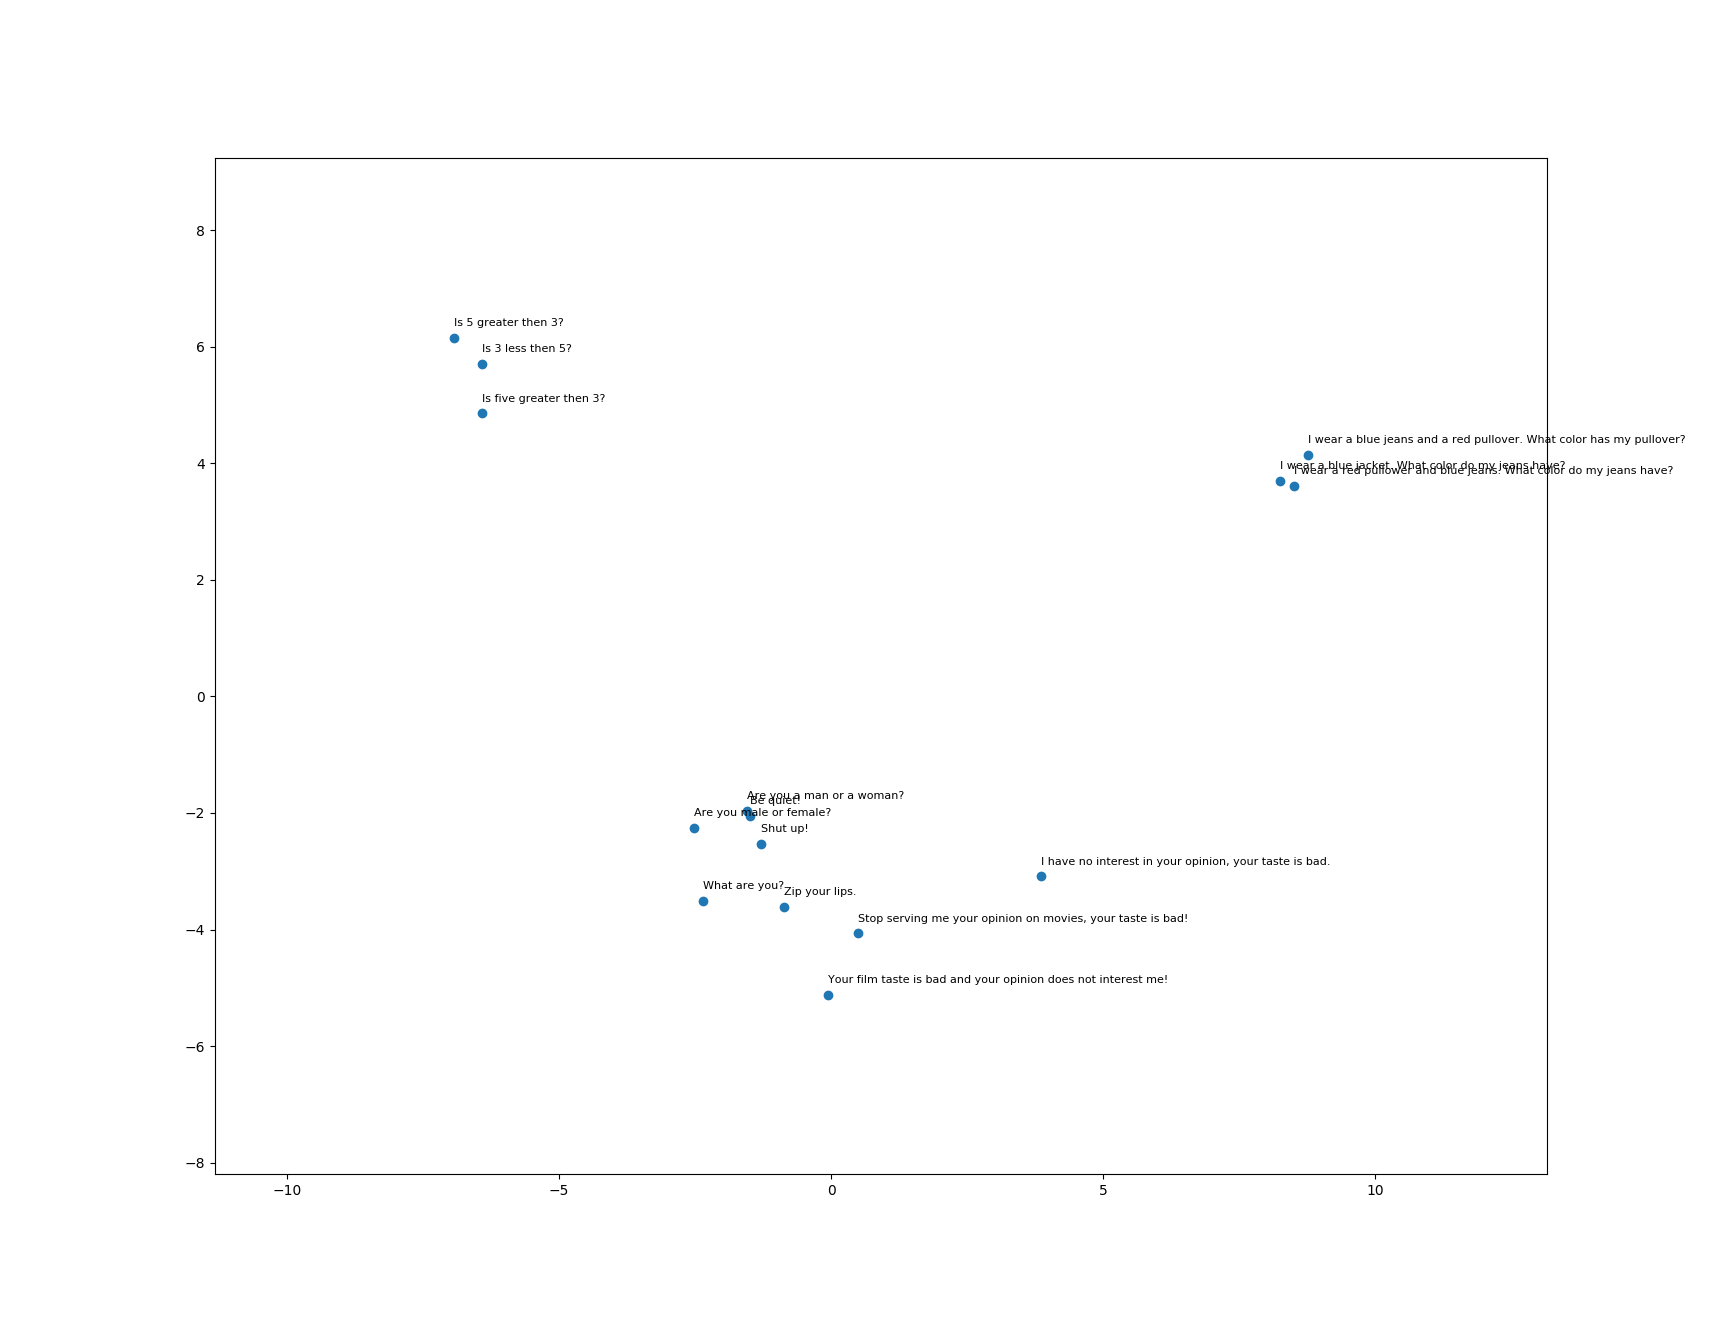
\includegraphics[width=14cm]{img/reddit_thought_vector_embeddings.png}
	\caption{The projected thought vectors for 15 different sentences when using the Reddit 2.0M model. PCA was used for the projection.}
	\label{results:thougth_vectors:embeddings:reddit}
\end{figure}

Both of the models seem to have no problems understanding direct sentences where the content is unambiguous (e.g. ``I have no interest in your opinion on movies, your taste is bad!''). This can be seen because similar sentences are clustered closely in the projected space. However, when it comes to curses and questions regarding the gender, the OpenSubtitles model starts to struggle, which can be seen by taking a look at the respective points in the projected space. The questions regarding the gender or the curses are scattered throughout the space, even though they should have been embedded closely to each other. The Reddit model seems to have less problems with this, as the embeddings for these sentences are clustered tighter. Interestingly, the Reddit model embeds the sentences with curses close to the sentences regarding the gender.

In general, it appears as the models have an understanding of these different sentences as most of the points are clustered, if they contain similar content. From this, we conclude that our models have, at least to a certain degree, an understanding of the meaning of utterances.

\section{Soft-Attention}
\label{results:soft_attention}
In the last part, we take a look at the soft-attention mechanism (see Chapter~\ref{fundamentals:soft_attention}) and analyze if the model benefits from its use by looking at the resulting attention weights. We do not expect significant advantages, as Vinyals and Le already notice in their paper~\cite{Vinyals:2015}. The visualizations are generated by feeding an utterance to our models and then visualizing the resulting attention weights (see Chapter~\ref{fundamentals:soft_attention}) in a heat-map over the different time steps of the decoding process. As utterances, we use three different examples, one general question, one mathematical question and an example which consists of two sentences with a relative pronoun in the second sentence, which refers to the subject of the first sentence.

We perform this analysis on the OpenSubtitles 3.0M and the Reddit 2.0M snapshots.

\paragraph{Attention Visualizations} The visualizations of the attention weights can be seen in Figures~\ref{results:attention:example3:opensubtitles-3M} and~\ref{results:attention:example3:reddit}. Additional visualizations of the same kind are located in Appendix~\ref{appendix:soft_attention}.

Clearly visible, the generated attention weights do not show a significant alignment with important words from the input utterance. For example, when looking at the input utterance ``anna is 18 years old. how old is she?'' (Figure~\ref{results:attention:example3:reddit}), we would expect that the decoder would place a large attention weight on the thought vector when the actual age of the person is processed. However, this is not the case for any of the output words.

\begin{figure}[h]
	\centering
	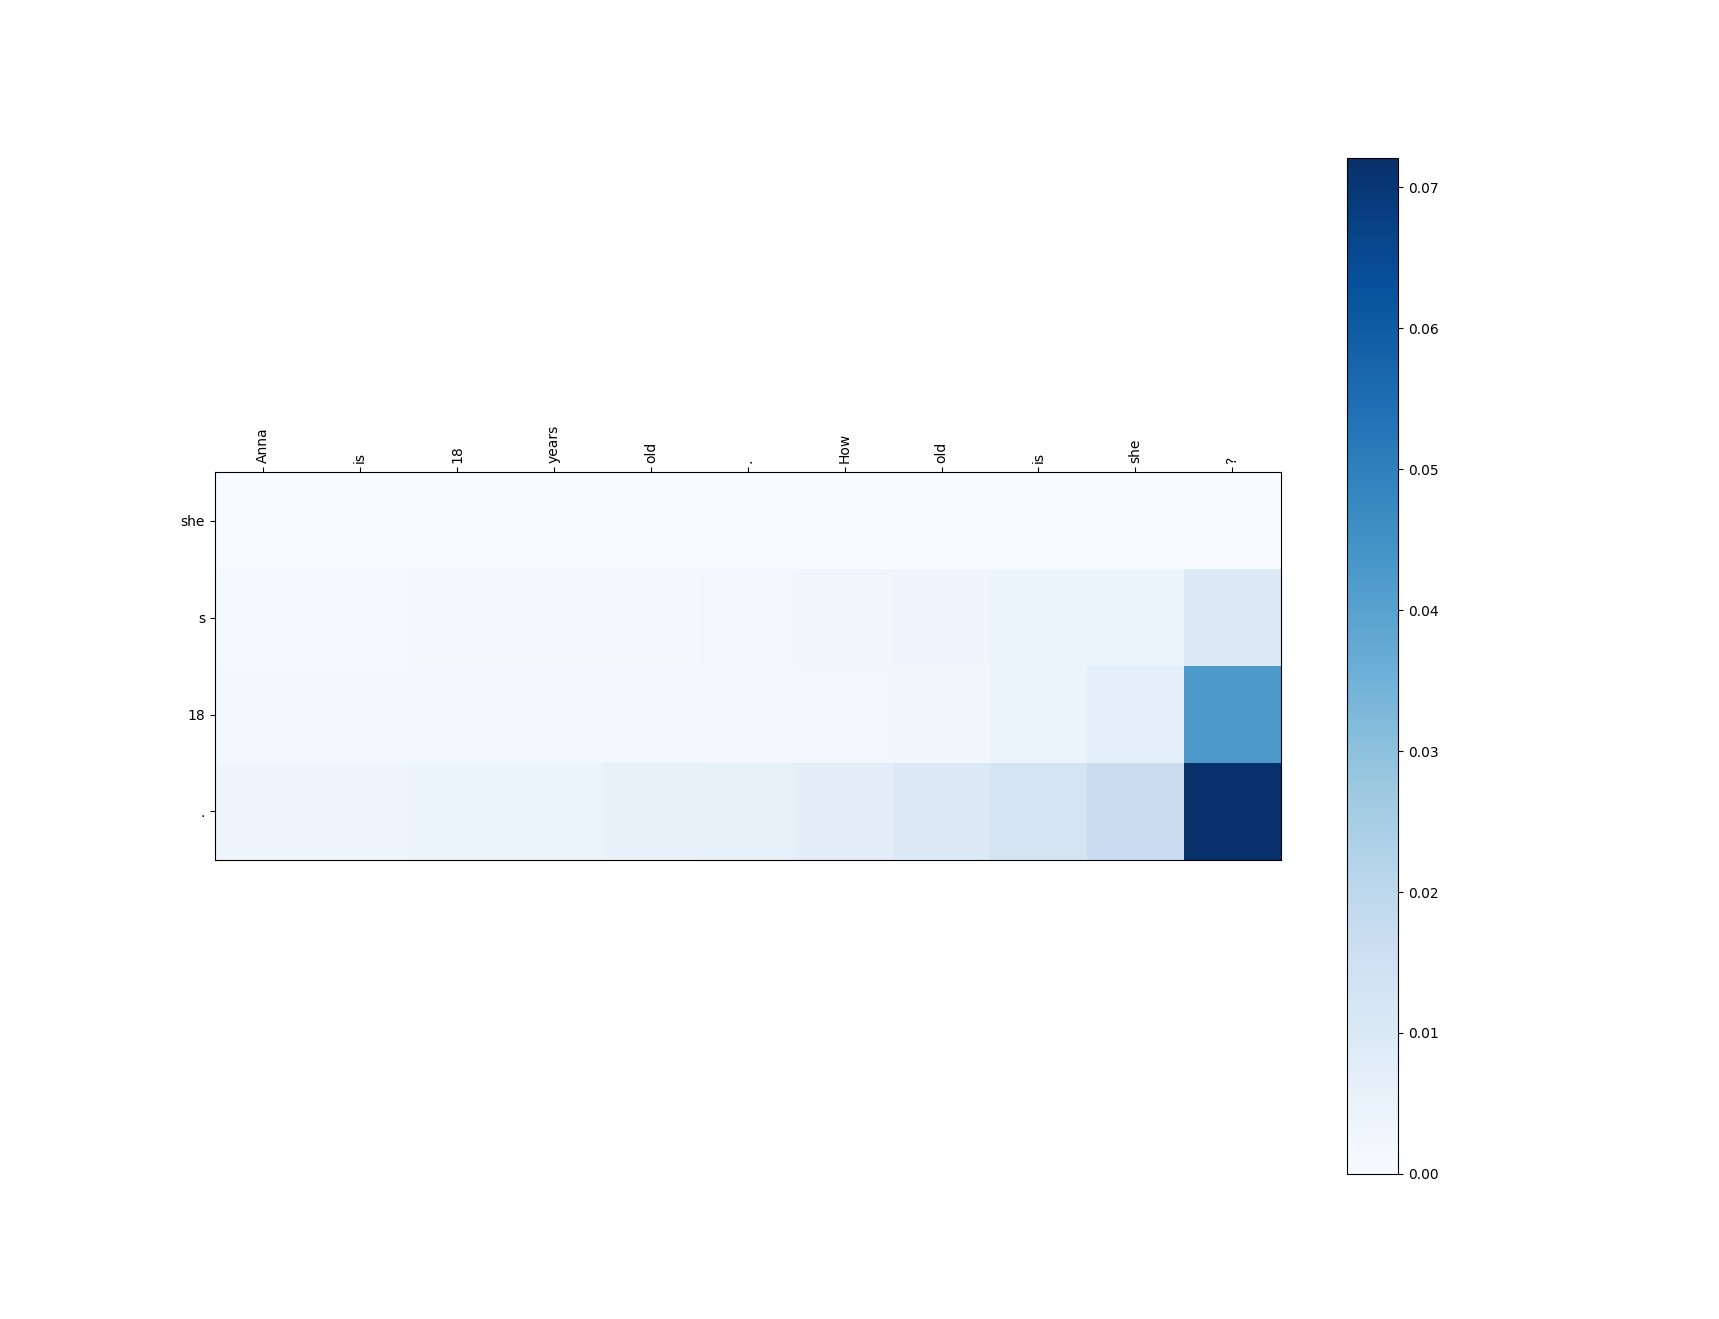
\includegraphics[width=10cm]{img/attention/attention_visualization3_reddit_2m.png}
	\caption{Visualization of the attention weights when using the utterance ``anna is 18 years old. how old is she?". On the x-axis, the input utterance is placed at the top of the chart from left to right. On the y-axis, the response from the model is placed from top to bottom. Each square in the heatmap corresponds to the attention weight the decoder computed for the thought vector of the corresponding word (x-axis) when producing the corresponding response word (y-axis). The Reddit 2.0M was used here.}
	\label{results:attention:example3:reddit}
\end{figure}

A second example, where attention does not compute meaningful alignments, is shown in Figure~\ref{results:attention:example3:opensubtitles-3M}. Here it is the same problem as before, the attention weights do not align with the important thought vectors from the input utterance.

\begin{figure}[h]
	\centering
	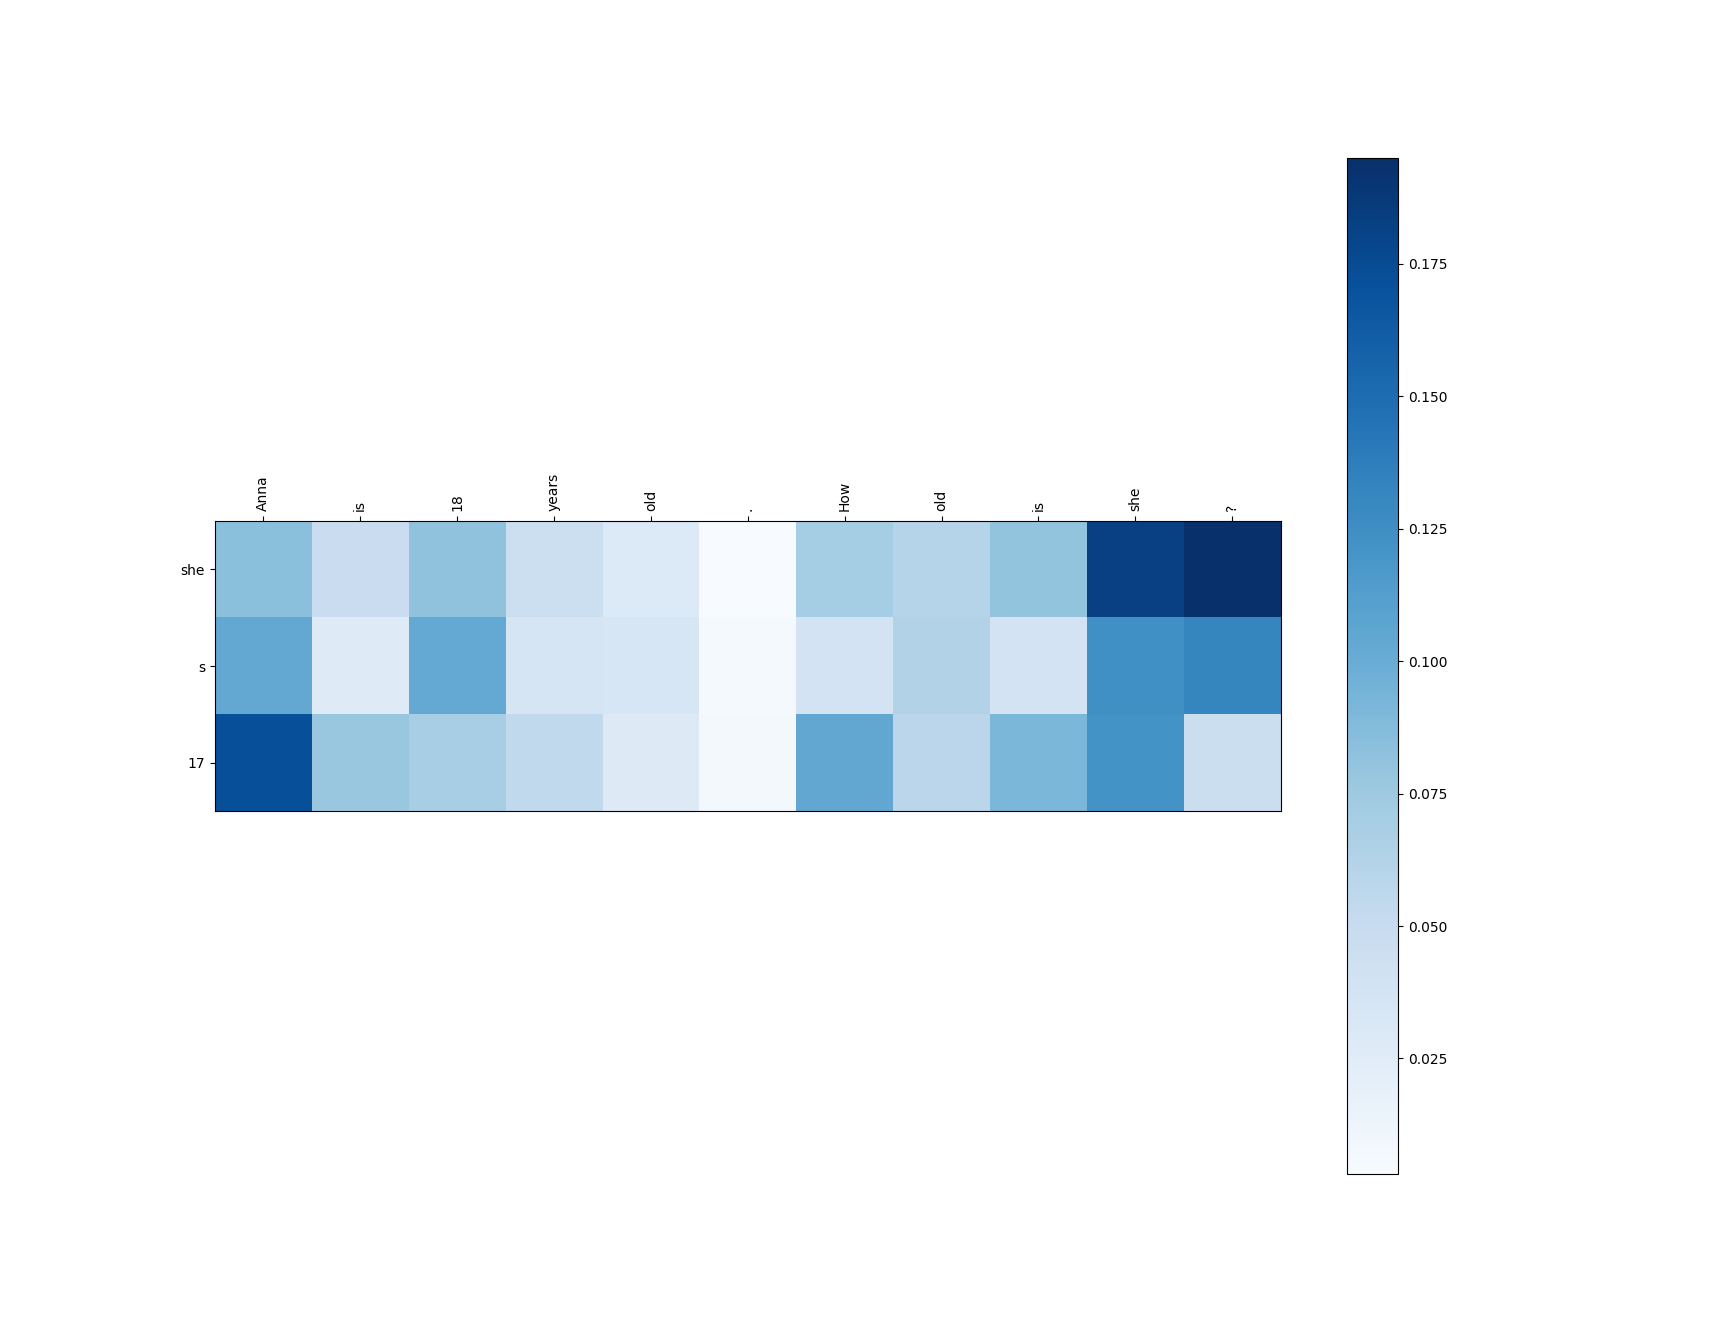
\includegraphics[width=10cm]{img/attention/attention_visualization3_OpenSubtitle-3M.png}
	\caption{Visualization of the attention weights when using the utterance ``anna is 18 years old. how old is she?". On the x-axis, the input utterance is placed at the top of the chart from left to right. On the y-axis, the response from the model is placed from top to bottom. Each square in the heatmap corresponds to the attention weight the decoder computed for the thought vector of the corresponding word (x-axis) when producing the corresponding response word (y-axis). The OpenSubtitles 3.0M was used here.}
	\label{results:attention:example3:opensubtitles-3M}
\end{figure}

From this quick analysis, we can reaffirm that the soft-attention mechanism does not seem to help to improve the decoders comprehension in conversational models. Our assumption is that it does not help because there are no clear alignments between the input and output as in other use-cases, such as machine translation or summary generation. This would explain why Vinyals and Le did not see an improvement with regard to loss and perplexity when using the soft-attention mechanism.

